\documentclass[]{beamer}

\usepackage[italian]{babel}
\usepackage{csquotes}
\usepackage[absolute,overlay]{textpos}
\usepackage{graphicx}
\usepackage[export]{adjustbox} % To align images side by side.
\usepackage[style=numeric-comp, minnames=2]{biblatex} % Required for the bibliography.
\usepackage{appendixnumberbeamer}

% Add bibliography sources.
\addbibresource{references.bib}

\definecolor{greenComplementary}{HTML}{75003A}

\hypersetup{
  colorlinks,
  allcolors=.,
  urlcolor=greenComplementary,
}

\setbeamertemplate{navigation symbols}{} % Remove navigation symbols.
\mode<presentation>{\usetheme{unimib-disco}}

\setbeamerfont{footnote}{size=\tiny}
\renewcommand{\cite}[1]{\footnote<.->[frame]{\fullcite{#1}}}
\setlength{\TPHorizModule}{\paperwidth}
\setlength{\TPVertModule}{\paperheight}

\title{Apprendimento per rinforzo multi-agente per la distribuzione del carico in servizi di edge computing FaaS}
\date{30 Ottobre 2024}
\author[]{Emanuele Petriglia}

% Compacted bibliography.
% Thanks to: https://tex.stackexchange.com/a/170312
\DeclareBibliographyAlias{article}{std}
\DeclareBibliographyAlias{book}{std}
\DeclareBibliographyAlias{booklet}{std}
\DeclareBibliographyAlias{collection}{std}
\DeclareBibliographyAlias{inbook}{std}
\DeclareBibliographyAlias{incollection}{std}
\DeclareBibliographyAlias{inproceedings}{std}
\DeclareBibliographyAlias{manual}{std}
\DeclareBibliographyAlias{misc}{std}
\DeclareBibliographyAlias{online}{std}
\DeclareBibliographyAlias{patent}{std}
\DeclareBibliographyAlias{periodical}{std}
\DeclareBibliographyAlias{proceedings}{std}
\DeclareBibliographyAlias{report}{std}
\DeclareBibliographyAlias{thesis}{std}
\DeclareBibliographyAlias{unpublished}{std}
\DeclareBibliographyAlias{*}{std}

\DeclareBibliographyDriver{std}{%
  \usebibmacro{bibindex}%
  \usebibmacro{begentry}%
  \usebibmacro{author/editor+others/translator+others}%
  \setunit{\labelnamepunct}\newblock
  \usebibmacro{title}%
  \newunit\newblock
  \usebibmacro{journal}%
  \newunit\newblock
  \usebibmacro{booktitle}%
  \newunit\newblock
  \usebibmacro{date}%
  \newunit\newblock
  \usebibmacro{finentry}}

\begin{document}

\begin{frame}[plain]
    \titlepage
\end{frame}

\begin{frame}[plain]
    \frametitle{Indice dei contenuti}
    \tableofcontents[hideallsubsections]
\end{frame}

\section{Introduzione}

\begin{frame}{Function as a Service (FaaS) nell'edge computing}
    \begin{itemize}
        \item \textbf{Edge computing}: modello di elaborazione in prossimità all'utente finale.

        \medskip

        \item \textbf{FaaS}: paradigma che consente di creare ed eseguire applicazioni come insieme di funzioni.
    \end{itemize}

    \centering
     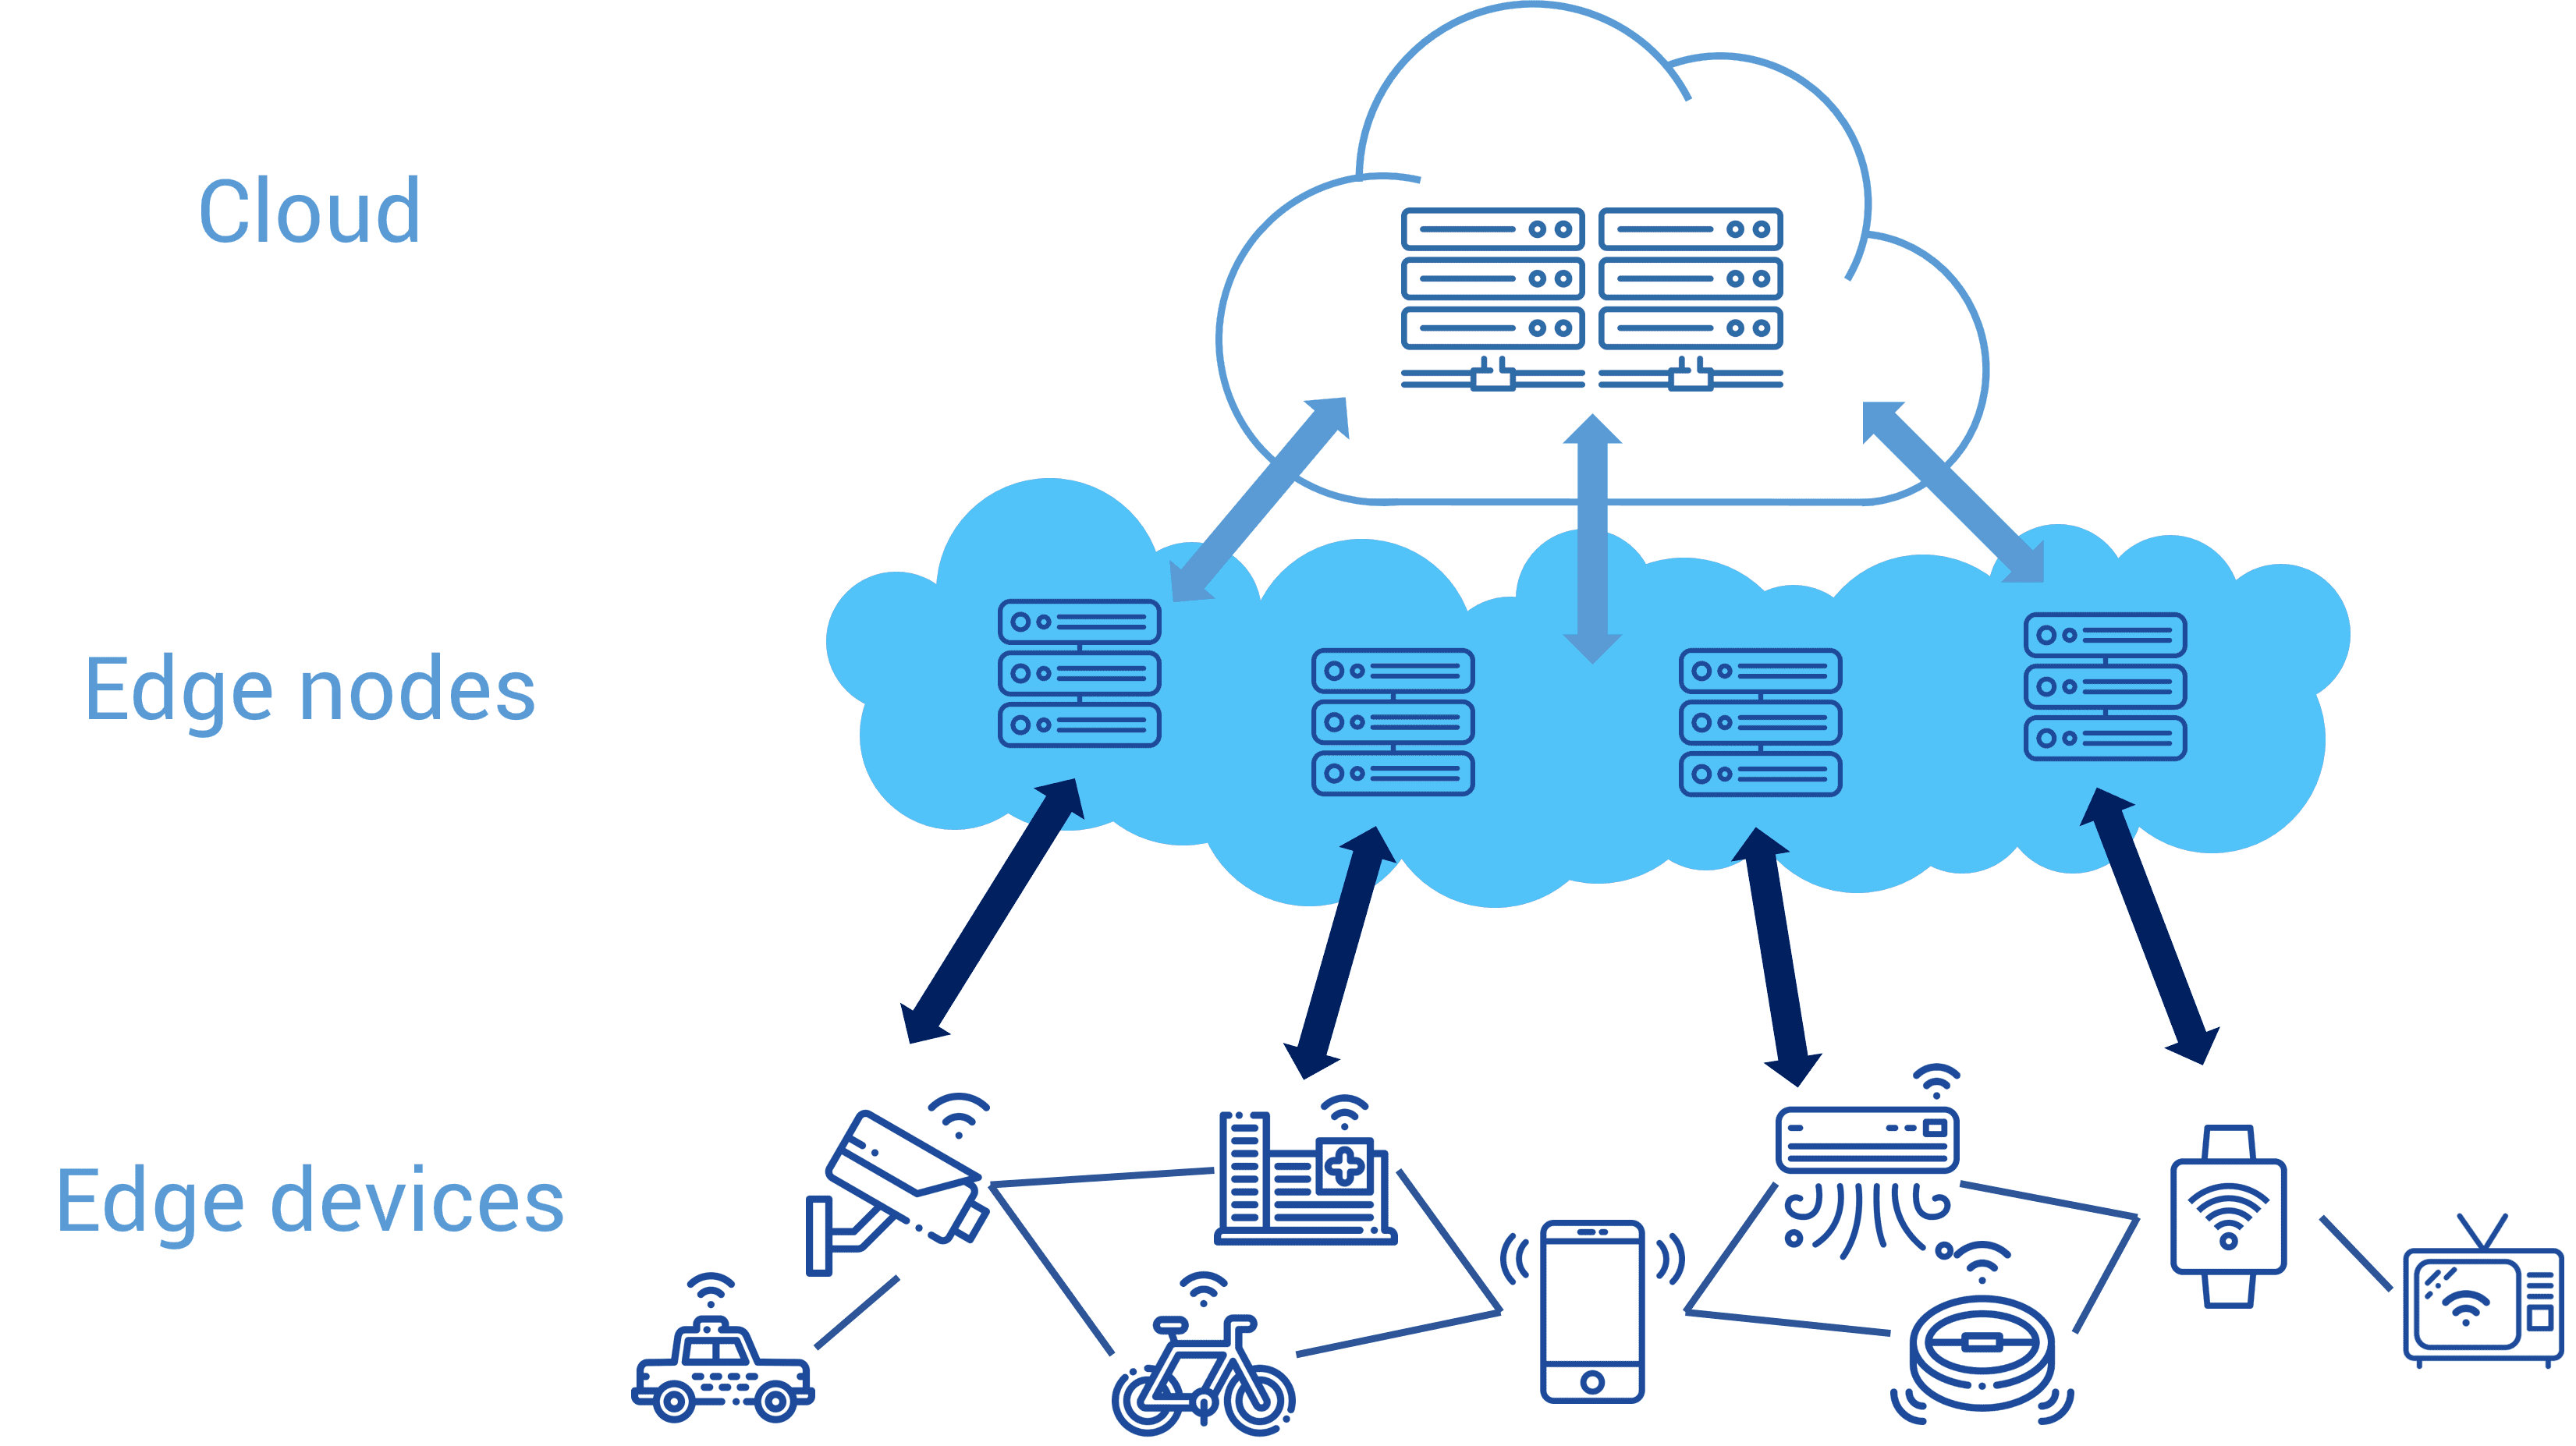
\includegraphics[width=.7\textwidth]{assets/slides/edge_computing.png}
     % https://www.alibabacloud.com/en/knowledge/what-is-edge-computing?_p_lc=1
\end{frame}

\begin{frame}{Decentralized DFaaS (DFaaS)}
    \begin{itemize}
        \item \textbf{DFaaS}\cite{Ciavotta2021}: architettura che unisce i modelli FaaS ed edge computing.

        \item Progettata per bilanciare autonomamente il carico in arrivo tra i nodi edge della rete.

        \item \textbf{Problema}: come bilanciare il carico in ingresso?
    \end{itemize}

    \centering
    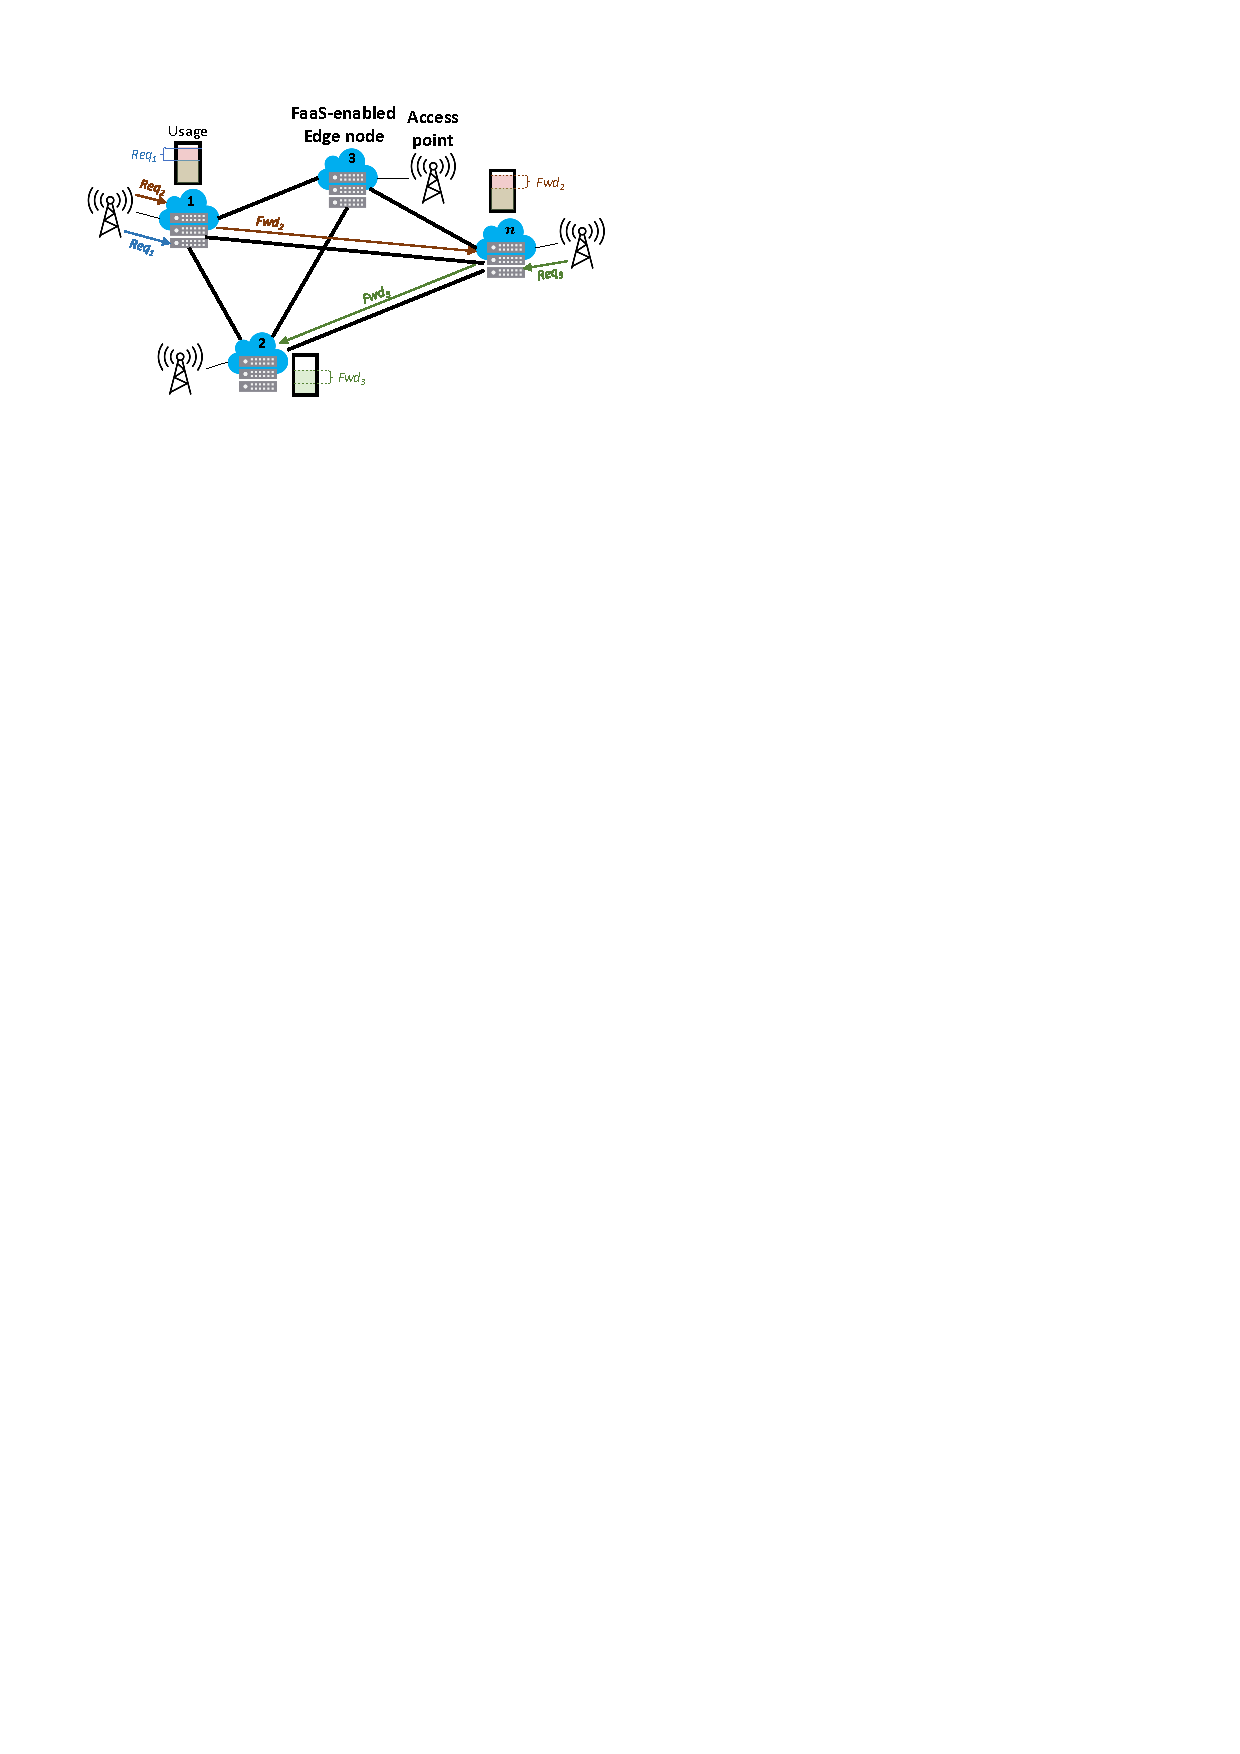
\includegraphics[width=.7\textwidth]{assets/2/dfaas_scenario.pdf}
\end{frame}

\begin{frame}{Apprendimento per Rinforzo (RL)}
    % \begin{itemize}
    %     \item \textbf{RL}:
    %     \begin{itemize}
    %         \item Spazio azioni
    %         \item Spazio osservazioni
    %         \item Funzione di ricompensa
    %     \end{itemize}
    % \end{itemize}
    % \centering
    % 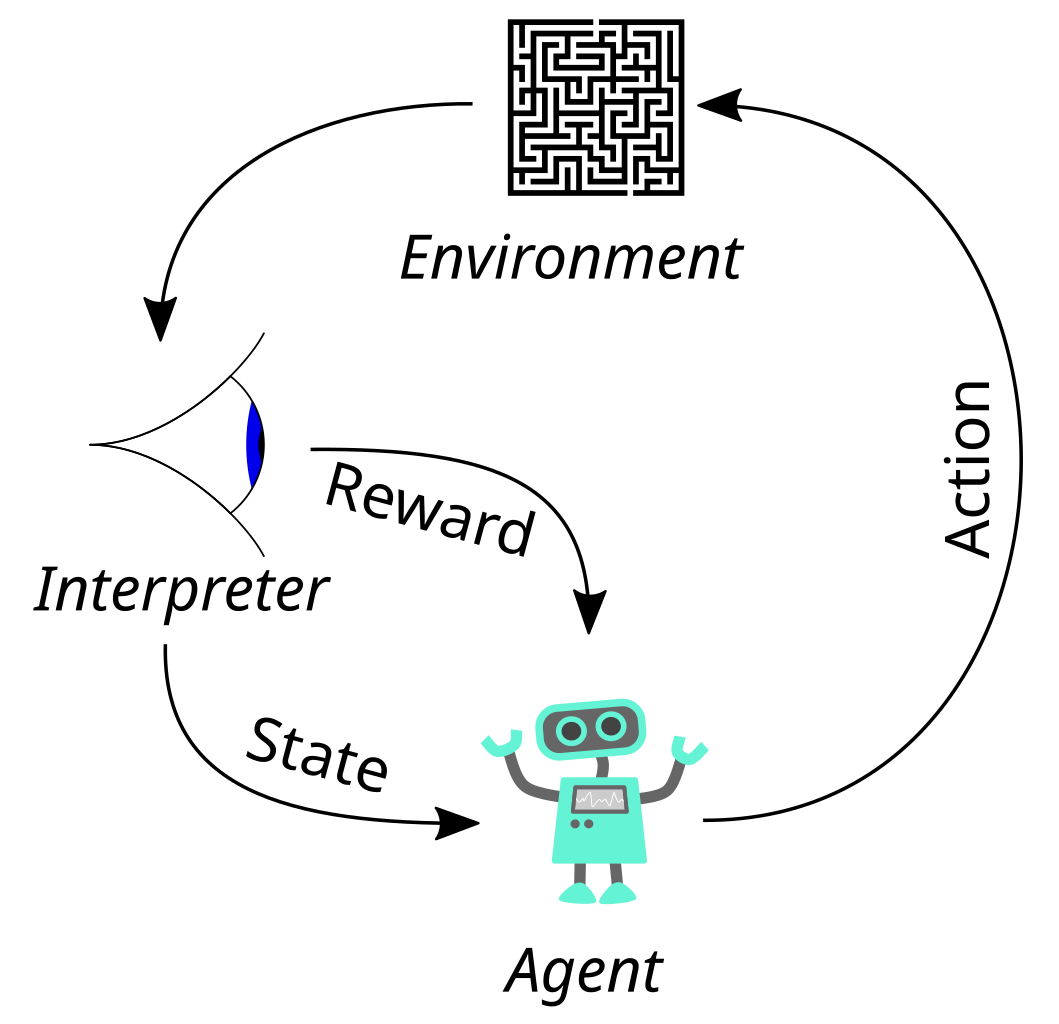
\includegraphics[width=.4\textwidth]{assets/2/rl_components.png}
    \begin{columns}
        \begin{column}{.7\textwidth}
            \begin{itemize}
                \item \textbf{RL}: Area interdisciplinare del machine learning e del controllo

                \medskip

                \item \textbf{Obiettivo}: massimizzare la ricompensa sul lungo periodo

                \medskip

                \item Per definire un problema di RL:

                \begin{enumerate}
                    \item Spazio azioni $\mathcal{A}$
                    \item Spazio osservazioni $\mathcal{S}$
                    \item Funzione di ricompensa $\mathcal{R}$
                \end{enumerate}
            \end{itemize}
        \end{column}
        \begin{column}{.4\textwidth}
            \centering
            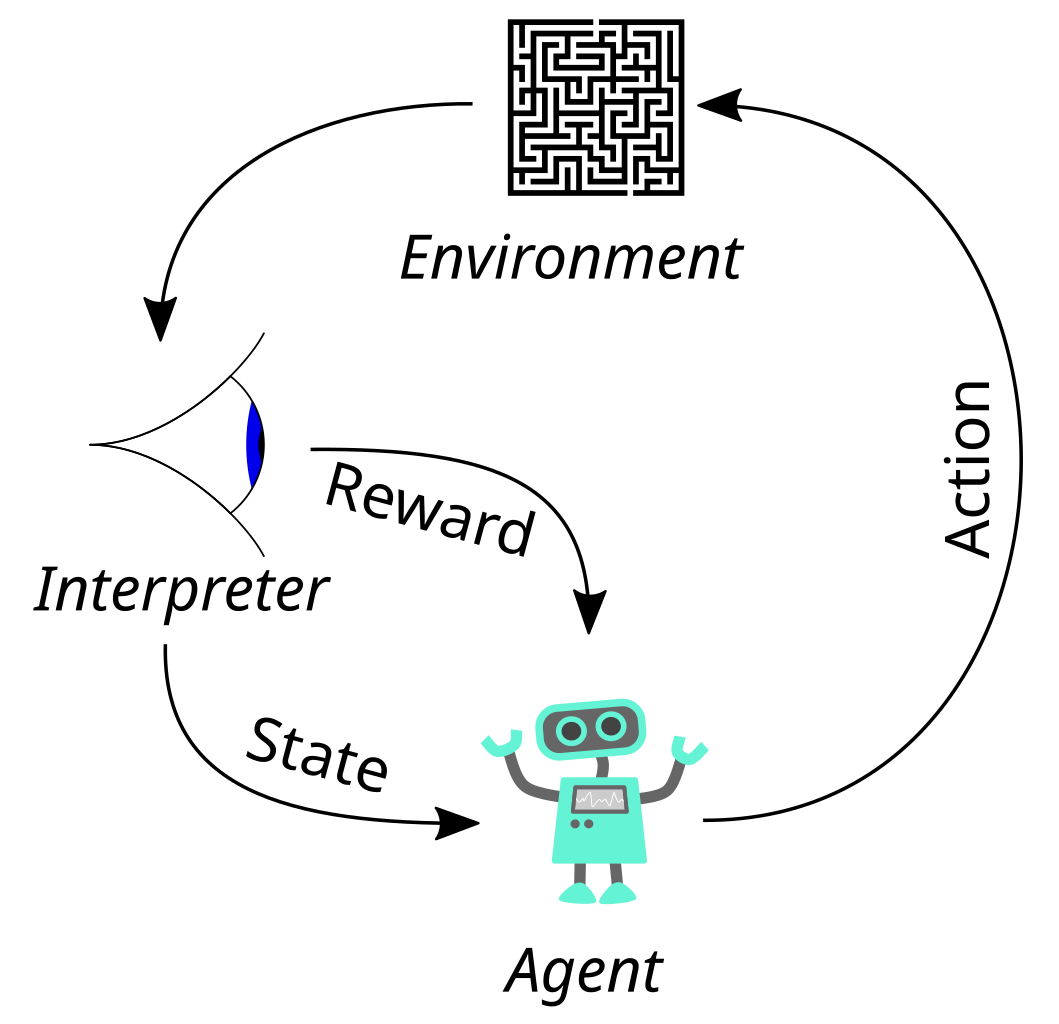
\includegraphics[width=.9\textwidth]{assets/2/rl_components.png}
        \end{column}
    \end{columns}
\end{frame}

\begin{frame}{Deep RL}
    \centering
    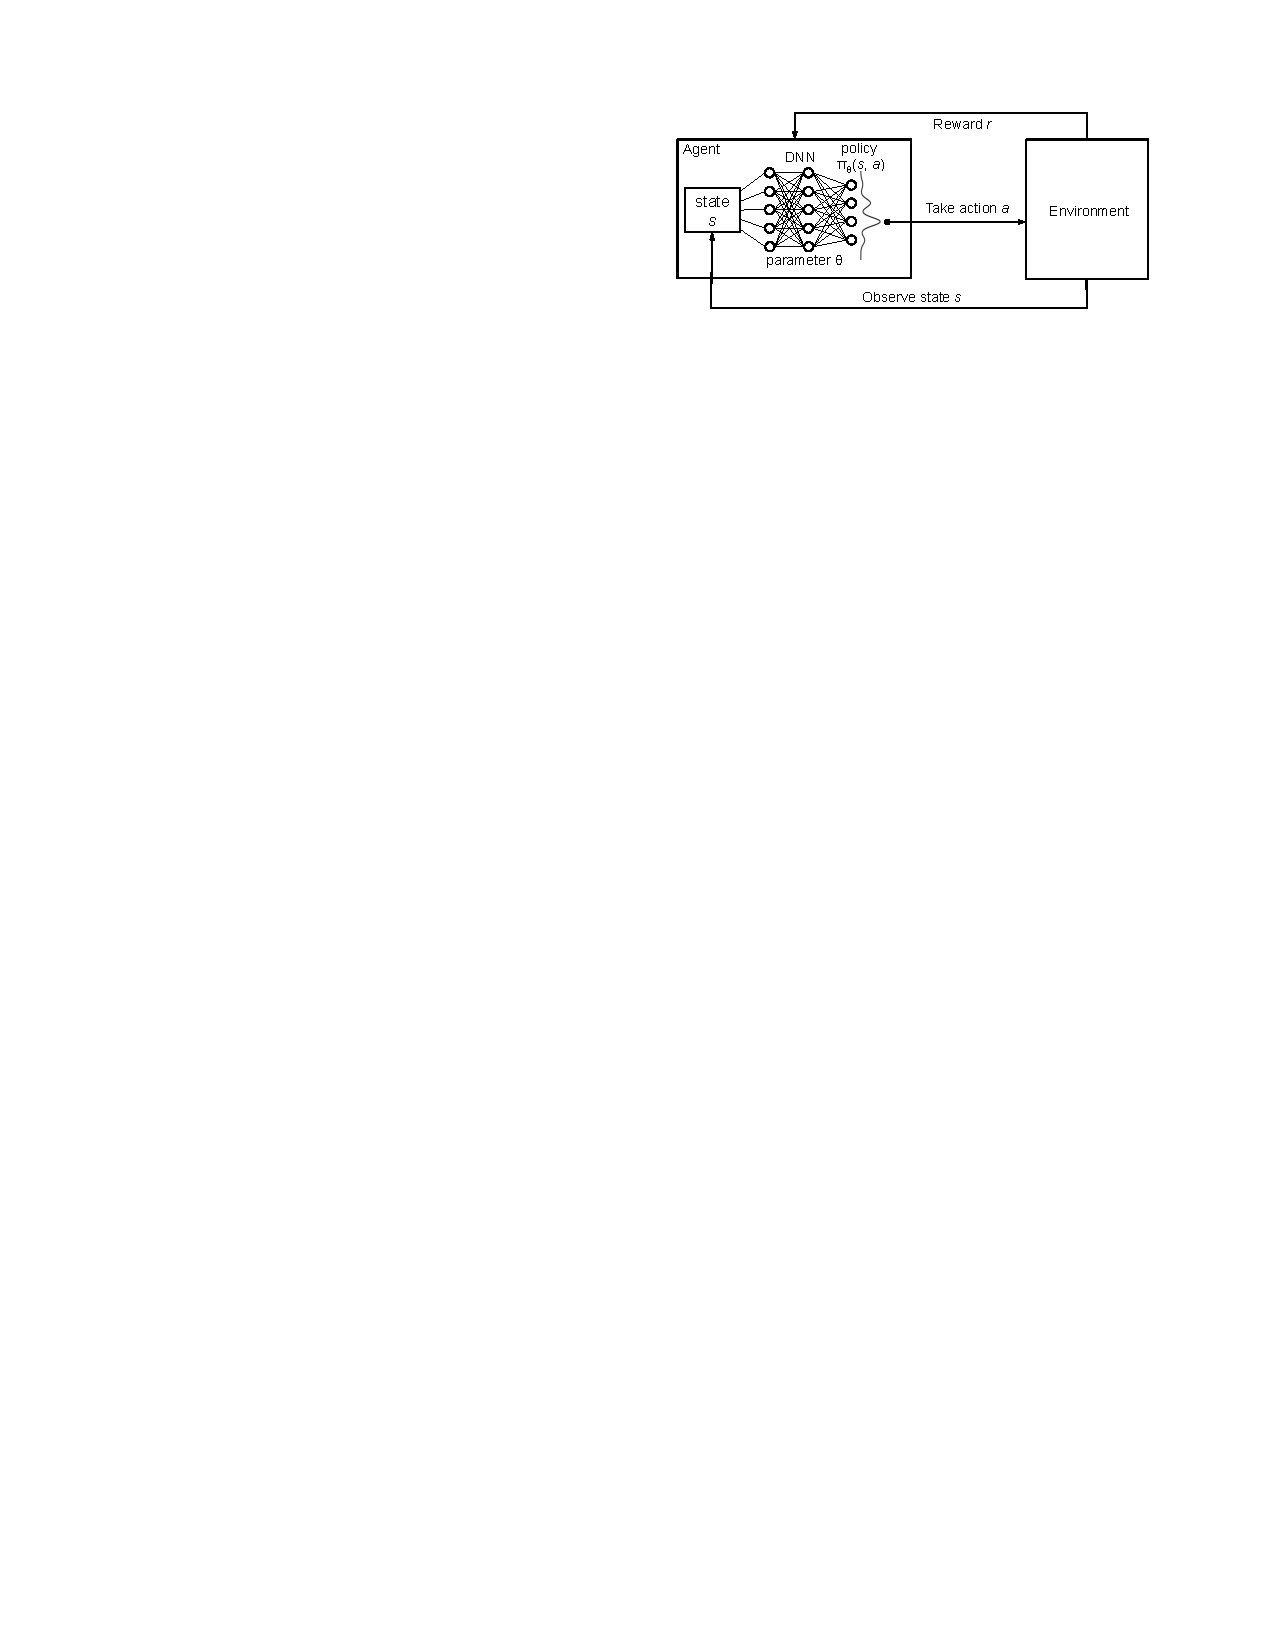
\includegraphics[width=\textwidth]{assets/slides/drl.pdf}
    % https://people.csail.mit.edu/alizadeh/papers/deeprm-hotnets16.pdf
\end{frame}

\begin{frame}{Apprendimento per Rinforzo Multi-Agente (MARL)}
    \centering
    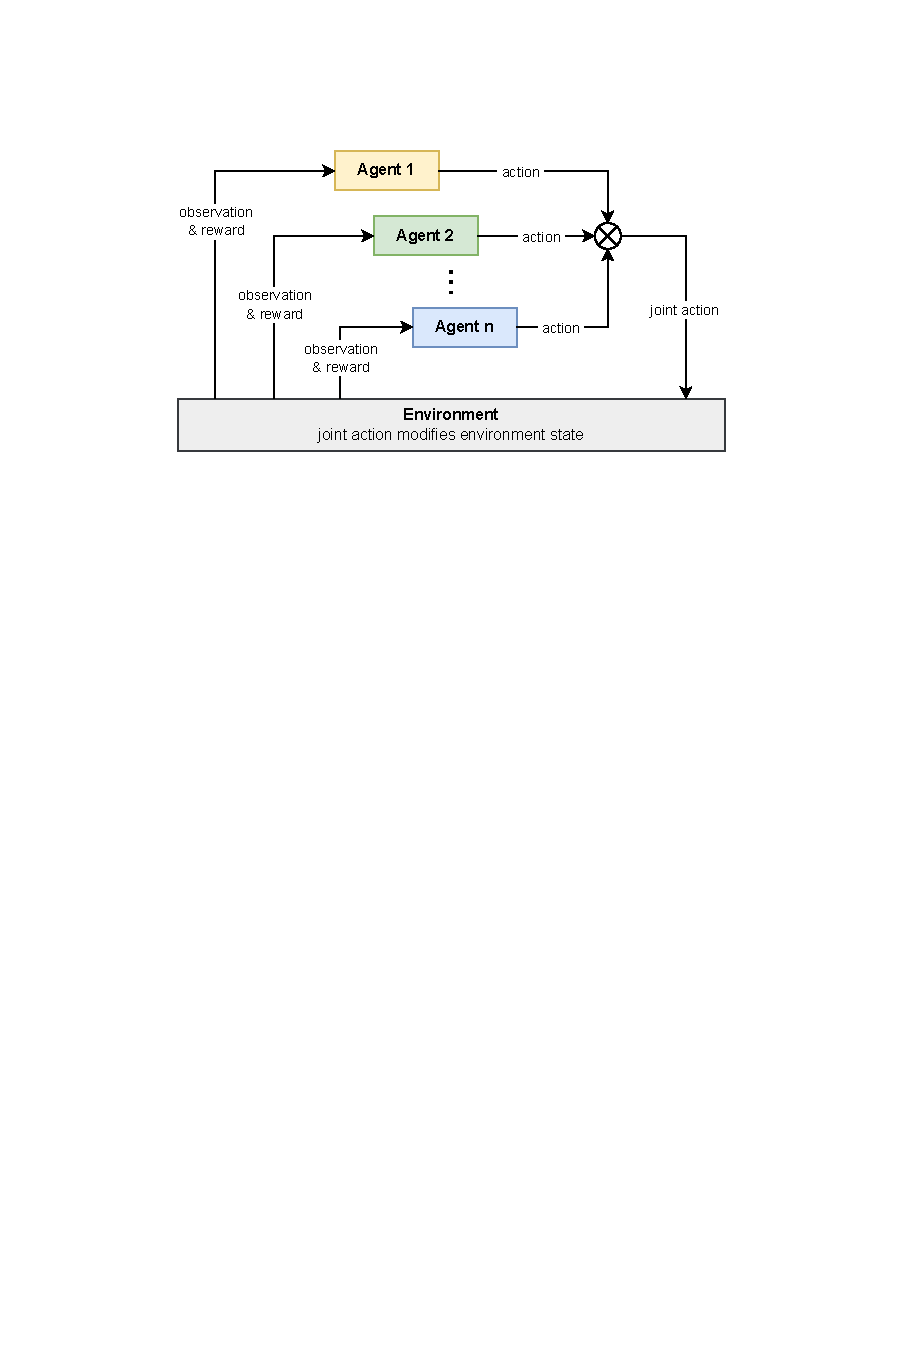
\includegraphics[width=.9\textwidth]{assets/2/rl_multi_agent_schematic.pdf}
\end{frame}

\begin{frame}{Problema affrontato}
    \begin{enumerate}
        \item Come modellare un problema MARL preliminare per la gestione del carico in ingresso in un sistema DFaaS?

        \vspace{1cm}

        \item L'approccio MARL è in grado di affrontare il problema allo scopo di processare più richieste possibili?
    \end{enumerate}
\end{frame}

\section{Modellazione degli ambienti}

\begin{frame}{Tre ambienti ad alto livello}
    \begin{columns}
        \begin{column}{.6\textwidth}
            \begin{enumerate}
                \vspace{.5cm}
                \item Simmetrico senza inoltro (``BASE'')
                \vspace{2.2cm}
                
                \item Asimmetrico (``ASYM'')
                \vspace{2.2cm}
                
                \item Simmetrico con inoltro (``SYM'')
            \end{enumerate}
        \end{column}
        \hspace{-1.7cm}
        \begin{column}{.7\textwidth}
            \centering
            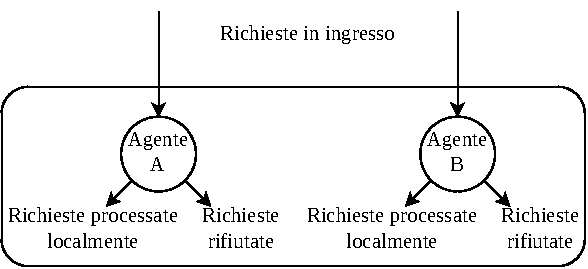
\includegraphics[width=.7\textwidth]{assets/4/1_sym_no_fw.pdf}
        
            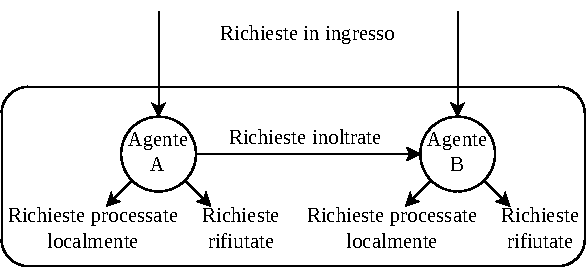
\includegraphics[width=.7\textwidth]{assets/4/2_asym.pdf}
        
            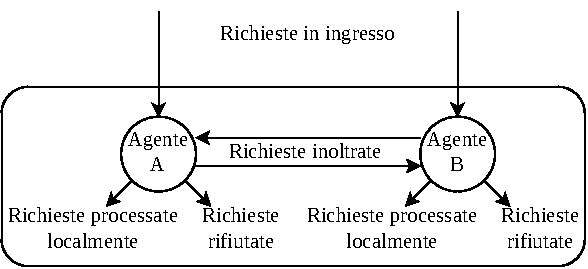
\includegraphics[width=.7\textwidth]{assets/4/3_sym_fw.pdf}
        \end{column}
    \end{columns}
\end{frame}

\begin{frame}{Spazio delle azioni}
    Ogni agente $a \in \mathcal{A}$ è una tupla:
    \begin{equation*}
        a = (p^{\textnormal{L}}, p^{\textnormal{F}}, p^{\textnormal{R}})
    \end{equation*}

    per cui:

    \begin{equation*}
        p^{\textnormal{L}} + p^{\textnormal{F}} + p^{\textnormal{R}} = 1
    \end{equation*}

    \centering
    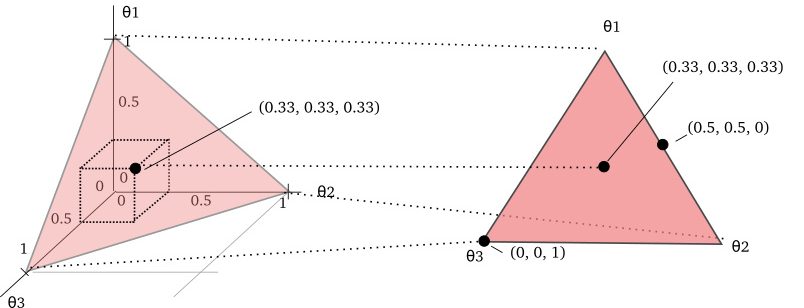
\includegraphics[width=.75\textwidth]{assets/4/simplex_5.png}
\end{frame}

\begin{frame}{Spazio delle osservazioni}
    Ogni agente $s \in \mathcal{S}$ è una tupla:
    \begin{equation*}
        s = (R^{\textnormal{IN}}, q^{\textnormal{FREE}}, s^{\textnormal{F}}, s^{\textnormal{FR}})
    \end{equation*}

    in cui:

    \begin{itemize}
        \item $R^{\textnormal{IN}}$: numero di richieste in ingresso al passo $t$

        \item $q^{\textnormal{FREE}}$: numero di slot disponibili in coda al passo $t$

        \item $s^{\textnormal{F}}$ sono il numero richieste inoltrate al passo $t-1$

        \item $s^{\textnormal{FR}}$ sono le richieste inoltrate ma rifiutate al passo $t-1$
    \end{itemize}
\end{frame}

\begin{frame}{Funzioni di ricompensa}
    \textbf{Due funzioni} di ricompensa in base alla tipologia di agente:

    \begin{enumerate}
        \item \textbf{Agente senza inoltro}: decresce la ricompensa alla presenza di richieste locali in eccesso o rifiutate

        \item \textbf{Agente con inoltro}: decresce la ricompensa all'aumentare delle richieste non processate in modo efficace
    \end{enumerate}

    \vspace{.5cm}

    Entrambe con codominio in $[0, 1] \in \mathrm{R}$.

    \begin{description}
        \item[\textbf{Priorità}] Proc. locale $\rightarrow$ Inoltro $\rightarrow$ Rifiuto

        \item[\textbf{Qualità}] Non ottimale $0 \longleftrightarrow 1$ Ottimale
    \end{description}
\end{frame}

\section{Algoritmo ``Proximal Policy Optimization''}

\begin{frame}{Proximal Policy Optimization (PPO)\cite{Schulman2017}}
    \begin{itemize}
        \item Algoritmo di Deep RL che supporta spazi d'azione continui
        
        \medskip

        \item Basato su architettura Actor-Critic:
        \begin{itemize}
            \item Rete Actor: che azione eseguire
            \item Rete Critic: valuta l'azione scelta
        \end{itemize}
        \centering
        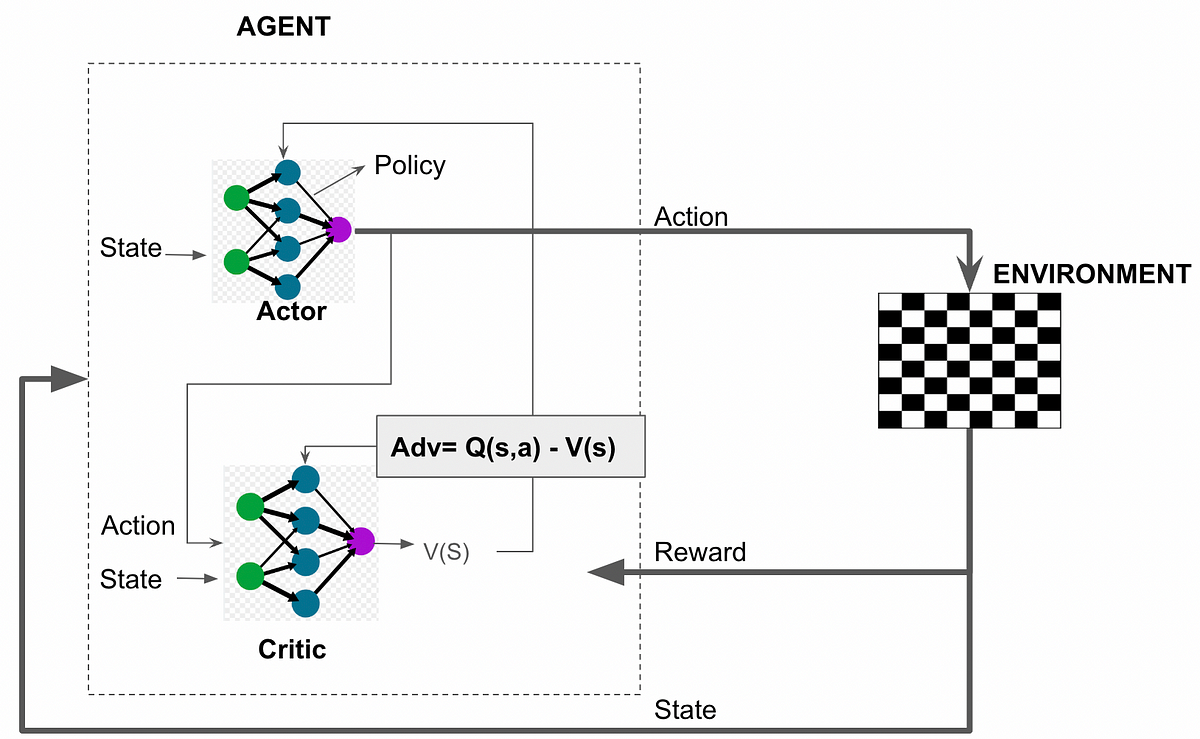
\includegraphics[width=.7\textwidth]{assets/slides/actor-critic.png}
        % https://arshren.medium.com/unlocking-the-secrets-of-actor-critic-reinforcement-learning-a-beginners-guide-3c5953b13551
    \end{itemize}
\end{frame}

\begin{frame}{Approcci MARL}
    \begin{itemize}
        \item Addestramento ed esecuzione centralizzati (a)

        \item \textbf{Addestramento ed esecuzione decentralizzati} (PPO) (b)

        \item \textbf{Addestramento centralizzato, esecuzione decentralizzata} (condivisione della rete Critic, PPO-CC) (c)
    \end{itemize}

    \medskip

    \centering
    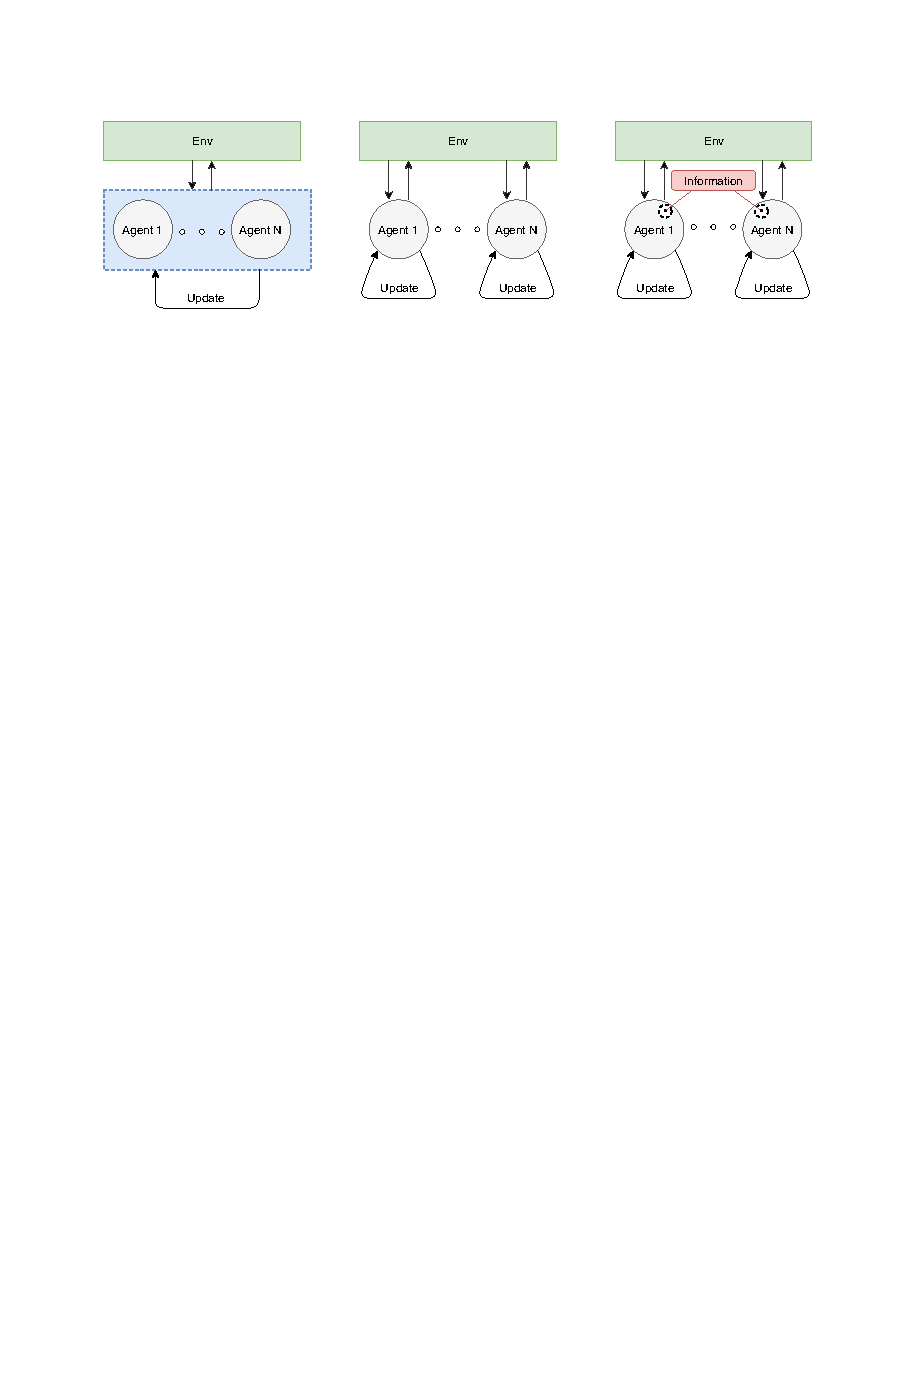
\includegraphics[width=\textwidth]{assets/slides/marl_approaches.pdf}
    % https://link.springer.com/article/10.1007/s10462-021-09996-w
    (a) \hspace{3.4cm} (b) \hspace{3.5cm} (c)
\end{frame}

\section{Sezione sperimentale}

\subsection{Configurazione e metodologia}

\begin{frame}{Configurazione degli ambienti e degli esperimenti}
    Configurazione ambienti:
    \begin{itemize}
        \item Ogni agente ha la stessa capacità di coda locale a 100
        \medskip

        \item Il carico in ingresso può variare in $[0, 150]$ per agente
        \medskip

        \item Ogni ambiente ha due agenti (in ASYM uno solo può inoltrare)
        \medskip

        \item Ambiente di tipo episodico da 288 passi
    \end{itemize}

    \medskip

    Configurazione esperimenti:
    \begin{enumerate}
        \item \textbf{Fase di addestramento}: agenti addestrati con PPO e PPO-CC per ogni scenario e ambiente

        \item \textbf{Fase di valutazione}: agenti valutati su 50 episodi per scenario
    \end{enumerate}
\end{frame}

\begin{frame}{Scenari}
    % \begin{columns}
    %     \begin{column}{.35\textwidth}
    %         \centering
    %         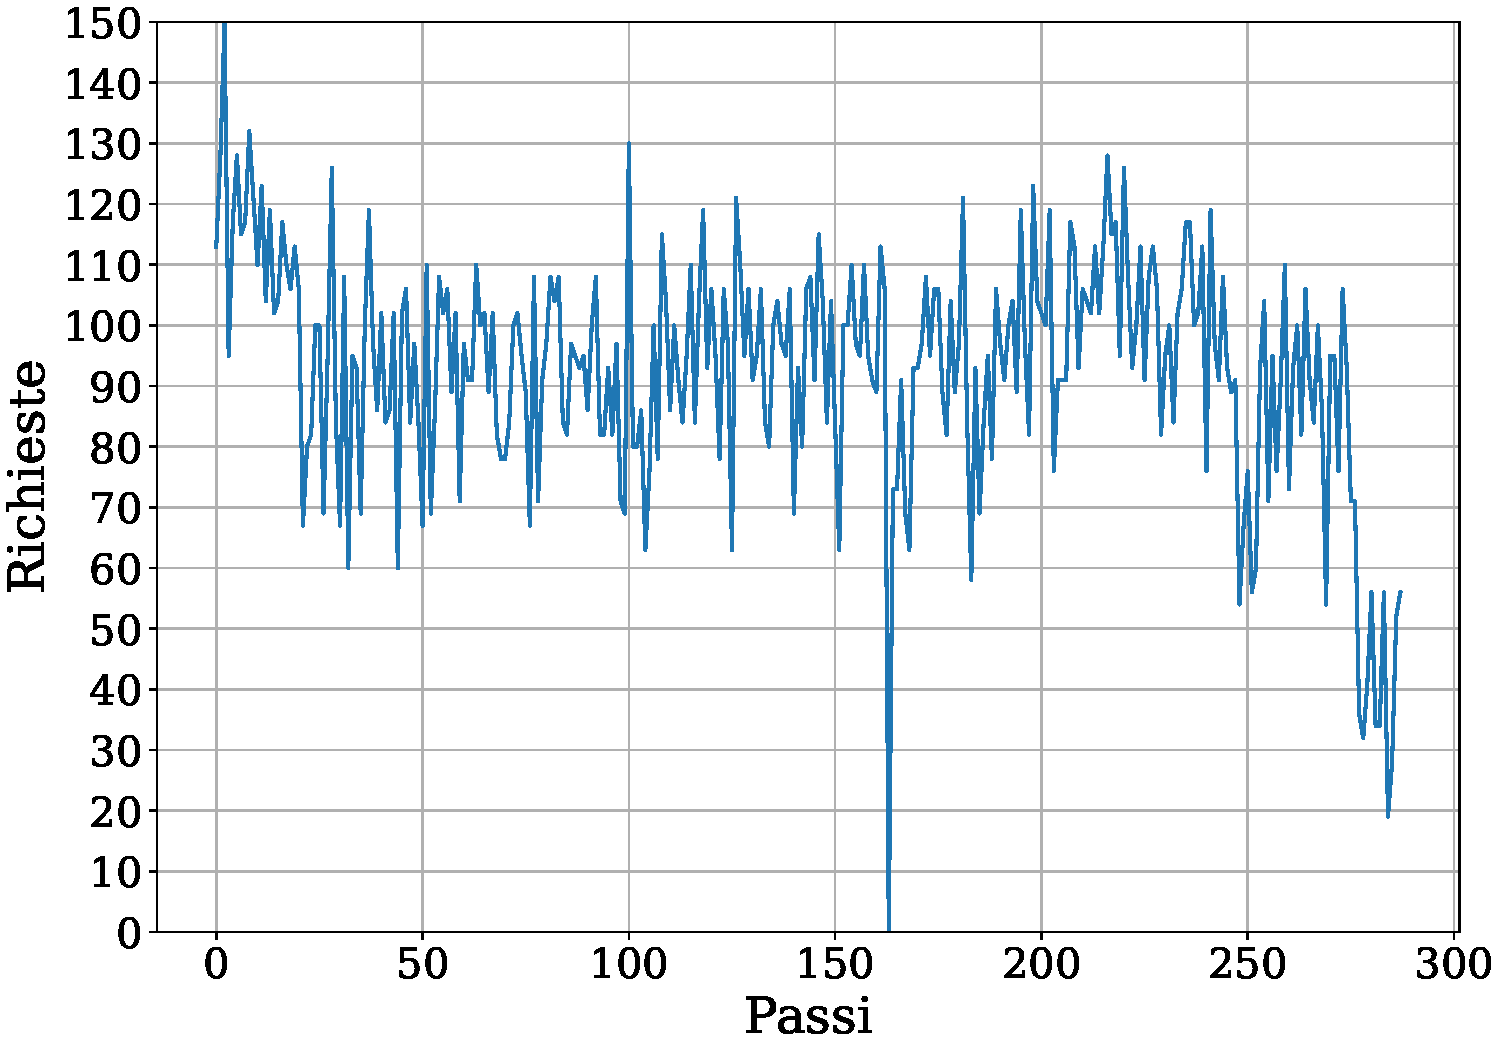
\includegraphics[width=\textwidth]{assets/5/requests_real_64425_single_agent.pdf}
    %         Reale
    %     \end{column}
    %     \begin{column}{.35\textwidth}
    %         \centering
    %         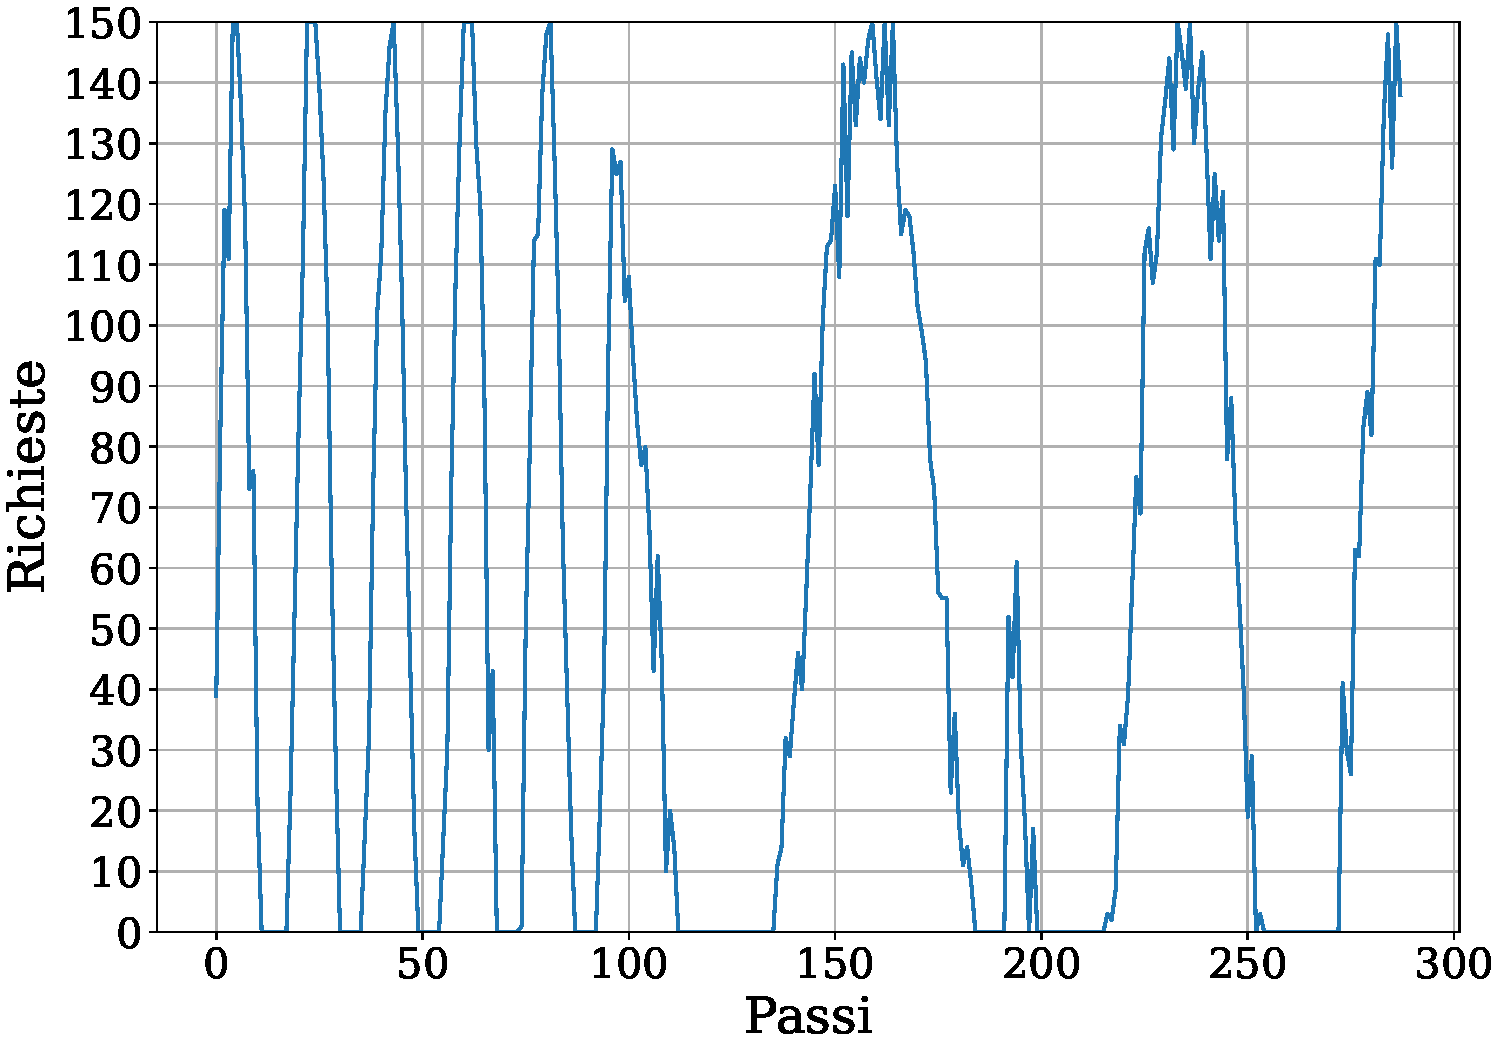
\includegraphics[width=\textwidth]{assets/5/requests_sinusoidal_64425_single_agent.pdf}
    %         Sintetico sinusoidale
    %     \end{column}
    %     \begin{column}{.35\textwidth}
    %         \centering
    %         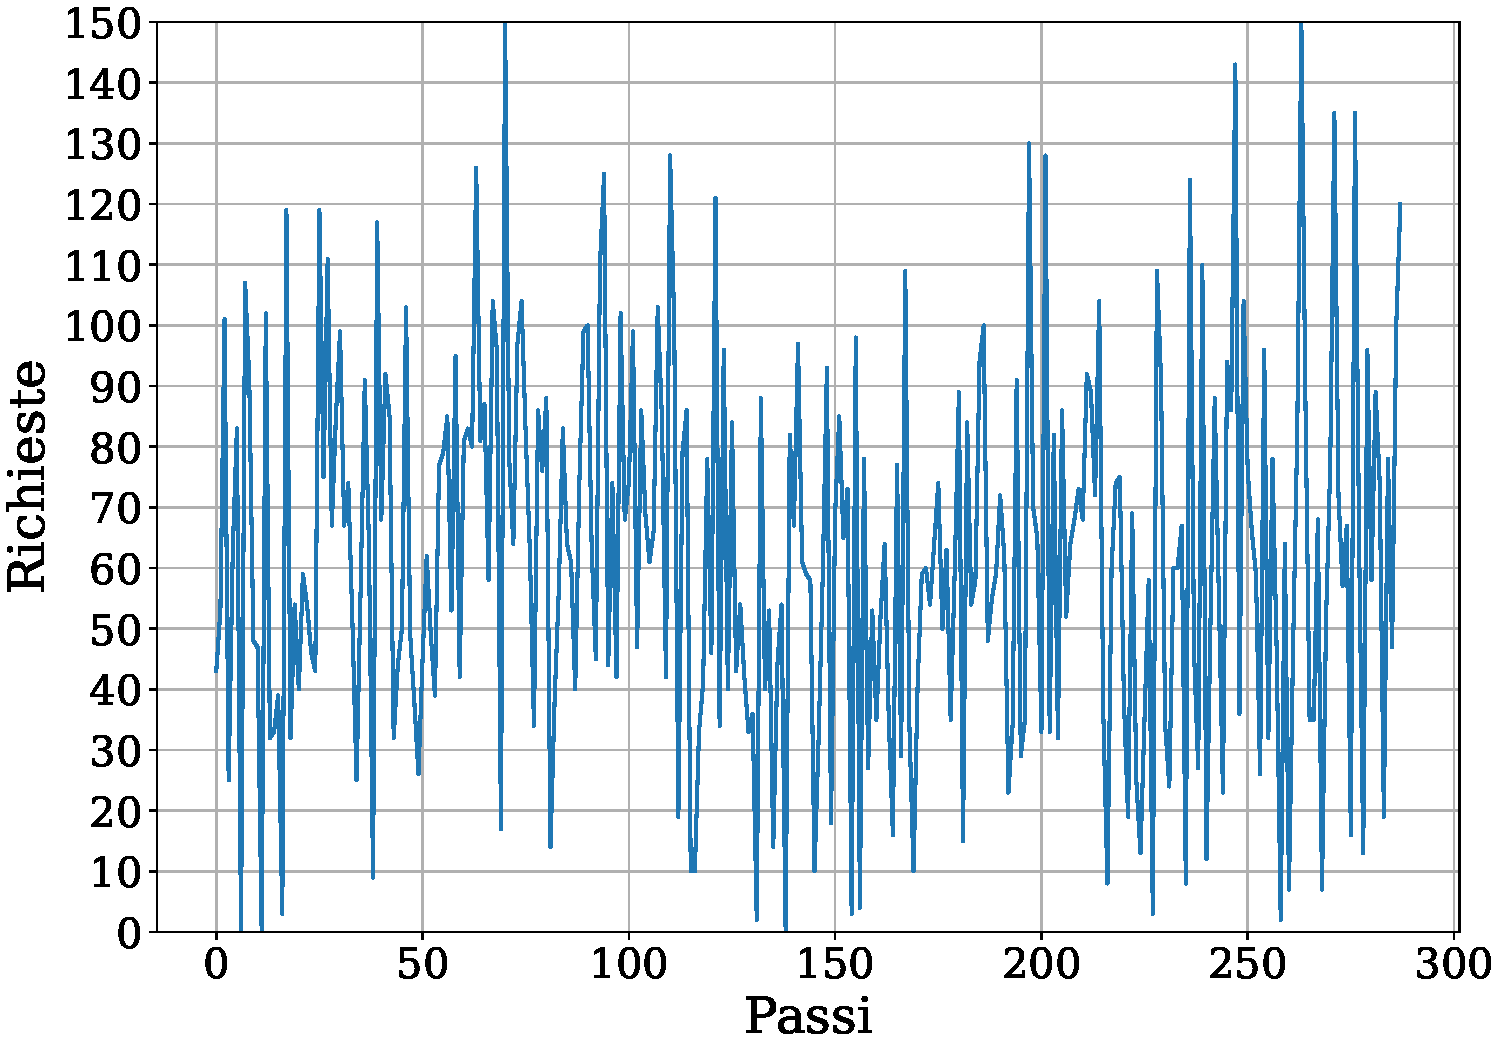
\includegraphics[width=\textwidth]{assets/5/requests_normal_64425_single_agent.pdf}
    %         Sintetico gaussiano
    %     \end{column}
    % \end{columns}
    \begin{columns}
        \begin{column}{.5\textwidth}           
            \centering
            Reale
            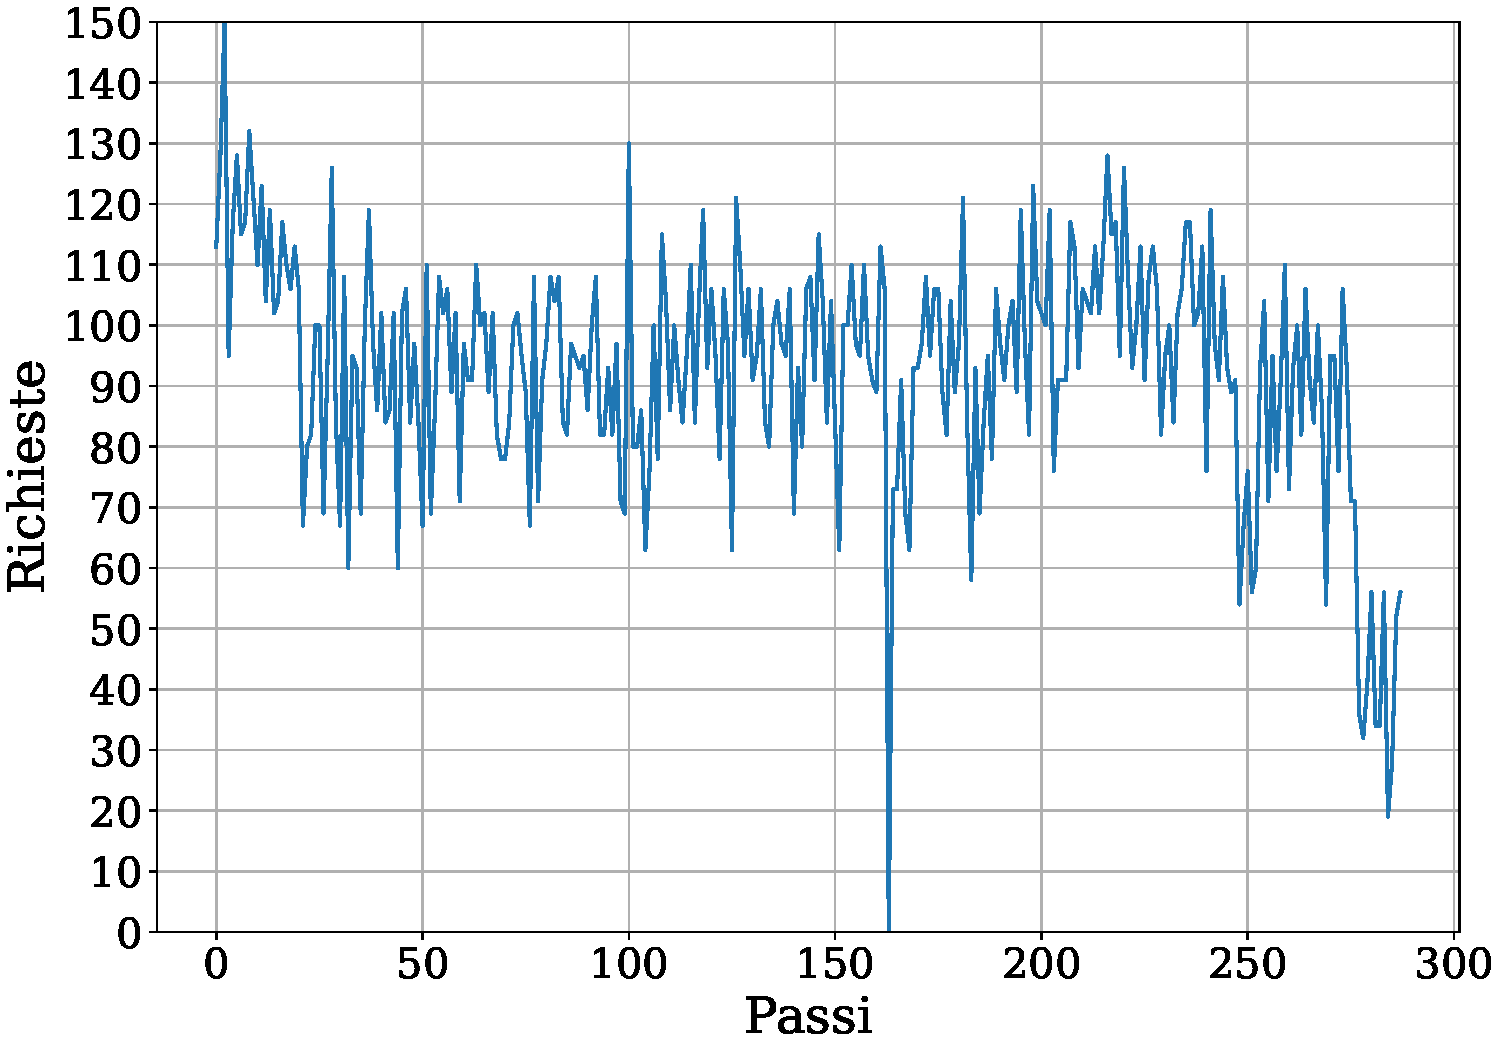
\includegraphics[width=5cm]{assets/5/requests_real_64425_single_agent.pdf}
        \end{column}
    \end{columns}

    \vspace{.4cm}

    \begin{columns}
        \begin{column}{.5\textwidth}
            \centering
            Sintetico sinusoidale
            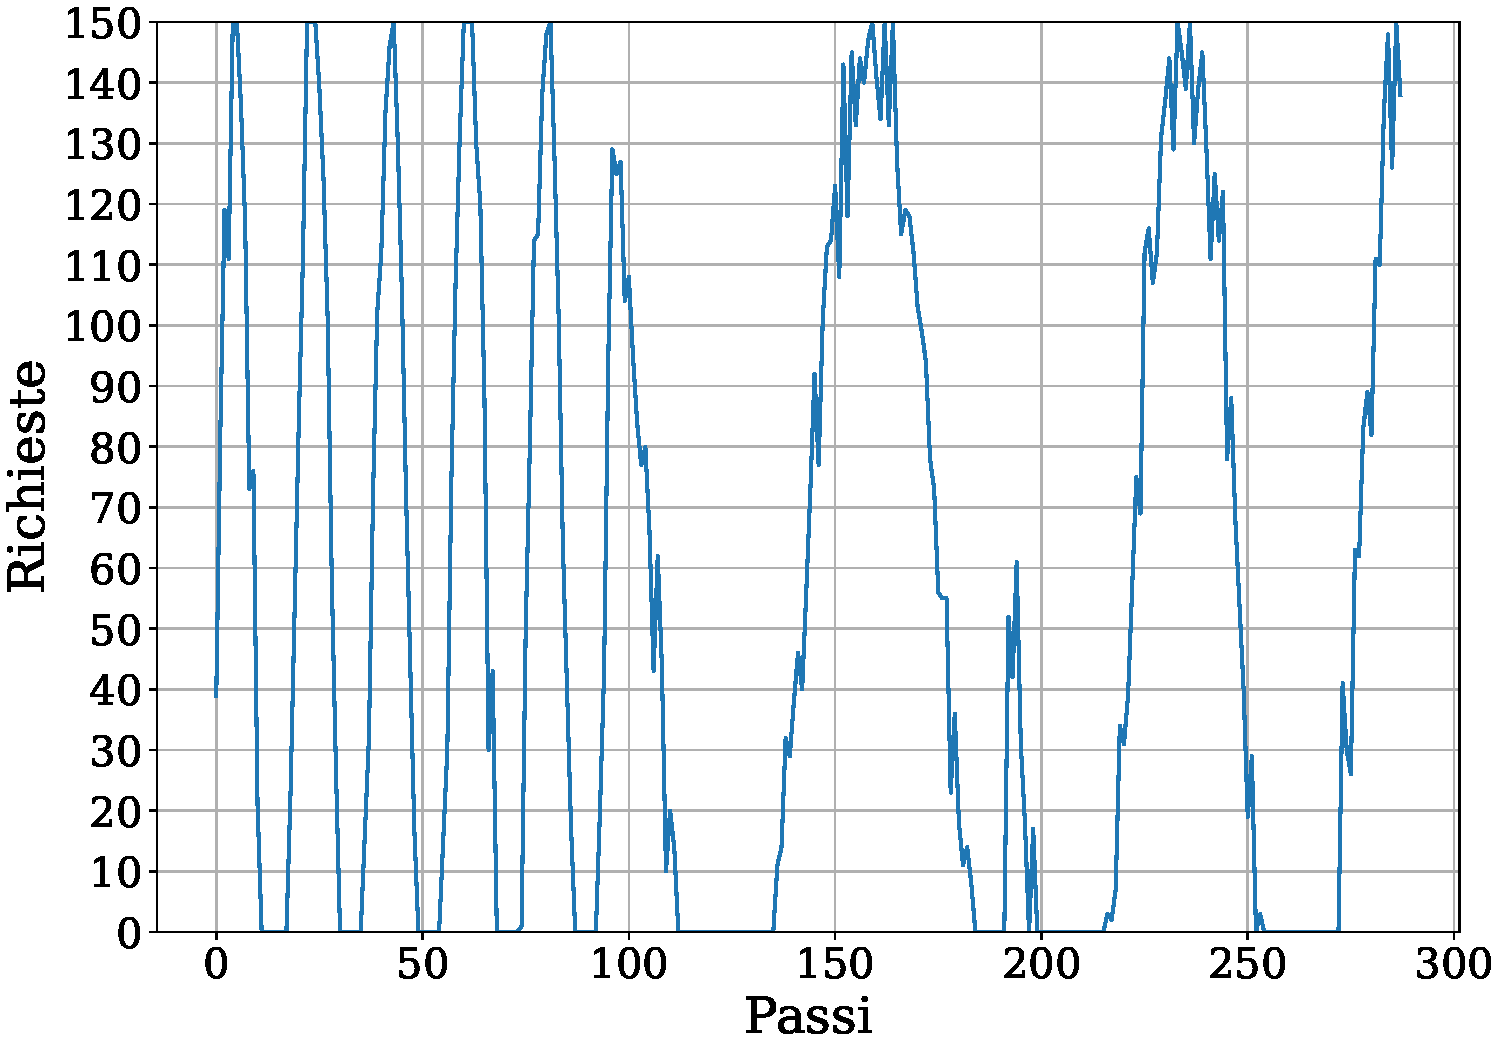
\includegraphics[width=5cm]{assets/5/requests_sinusoidal_64425_single_agent.pdf}
        \end{column}
        \begin{column}{.5\textwidth}
            \centering
            Sintetico gaussiano
            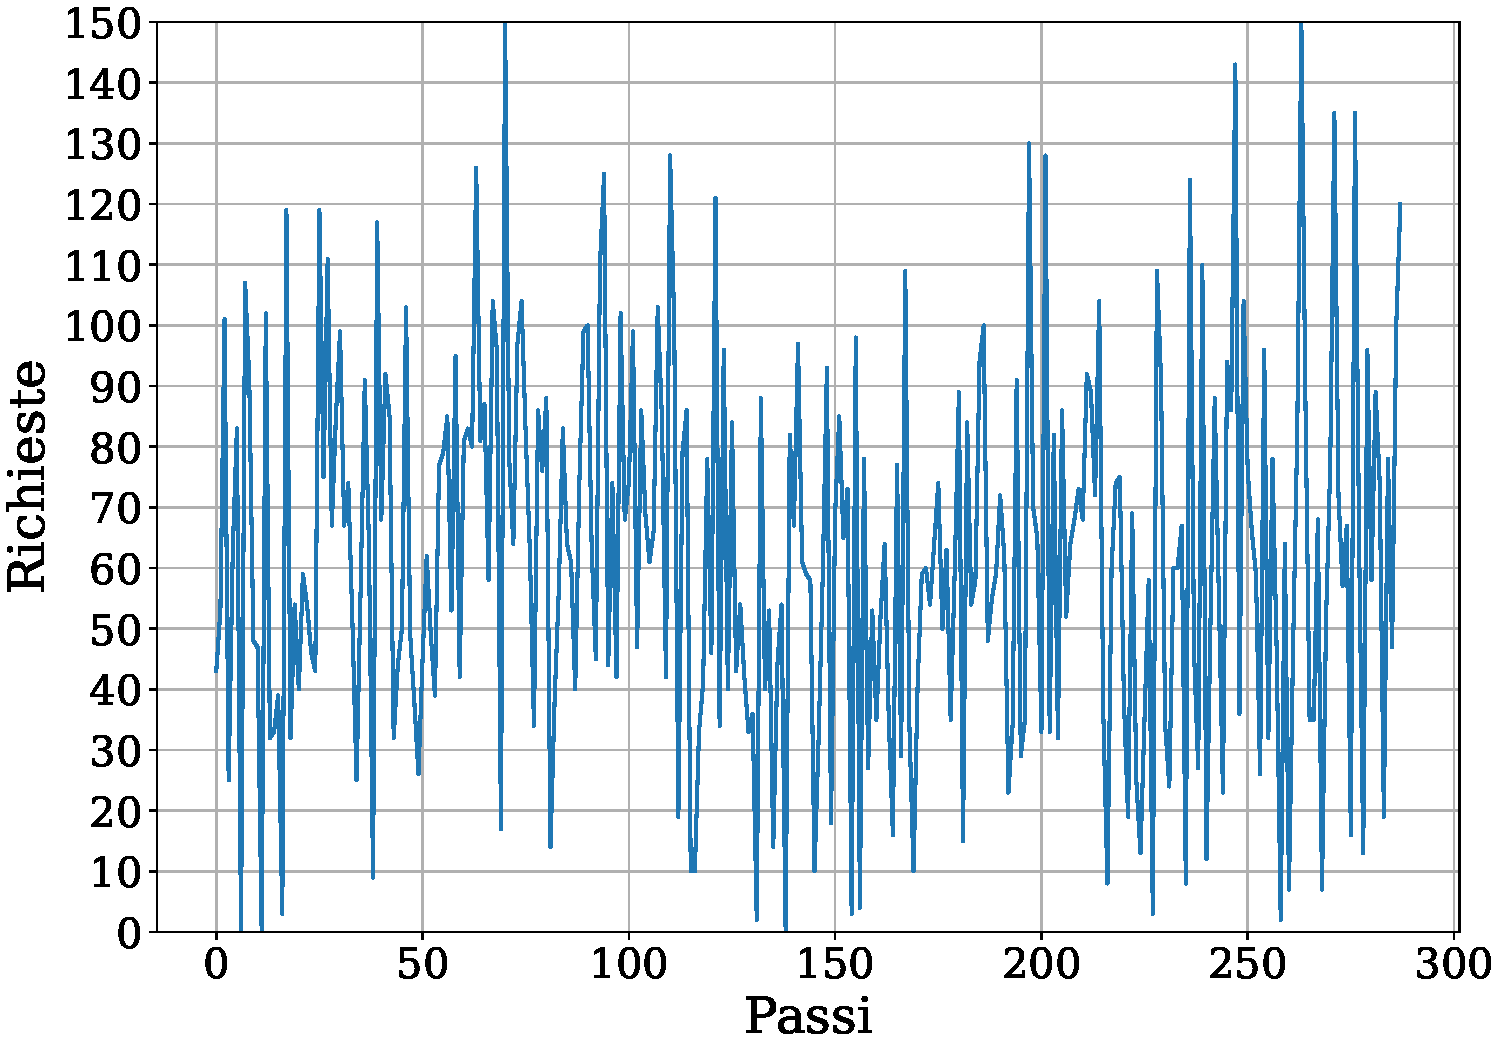
\includegraphics[width=5cm]{assets/5/requests_normal_64425_single_agent.pdf}
        \end{column}
    \end{columns}
\end{frame}

\subsection{Risultati preliminari}

\begin{frame}{Richieste processate}
    % \begin{columns}
    %     \begin{column}{.35\textwidth}
    %         \centering
    %         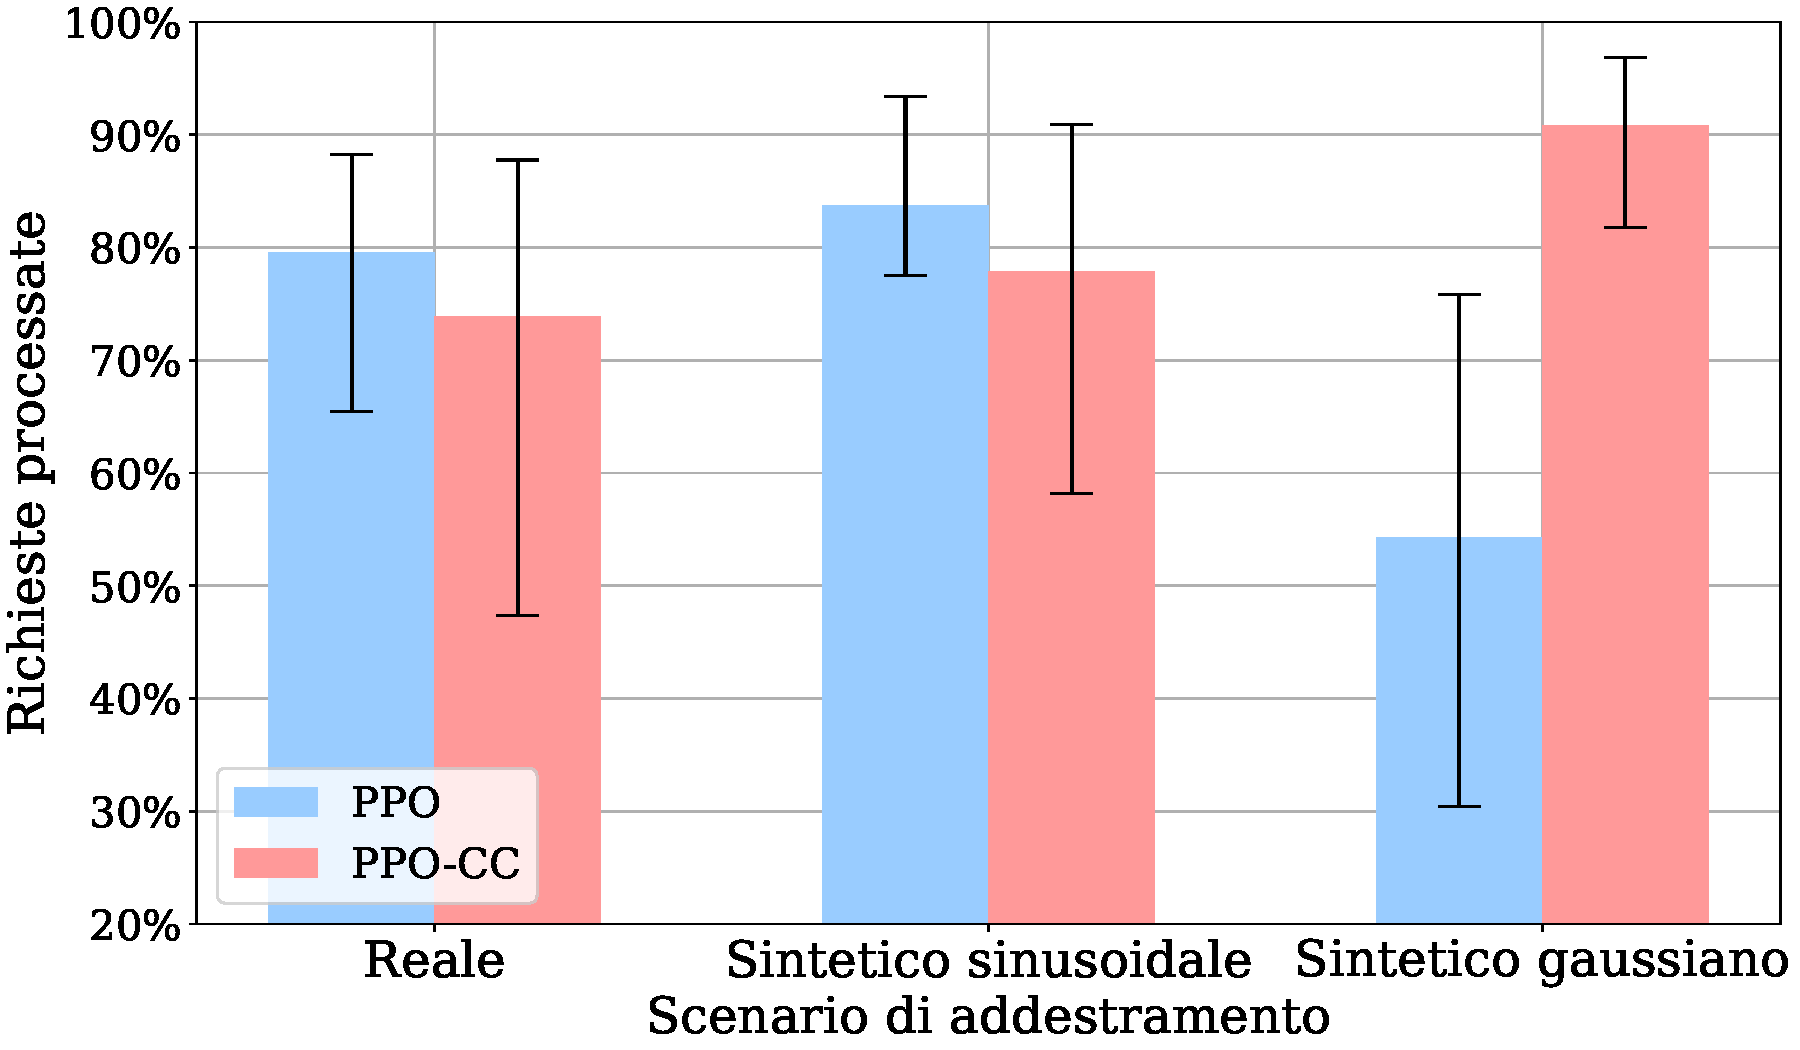
\includegraphics[width=\textwidth]{assets/5/results/eval_BASE_summary_processed_requests.pdf}
    %         Ambiente ``BASE''
    %     \end{column}
    %     \begin{column}{.35\textwidth}
    %         \centering
    %         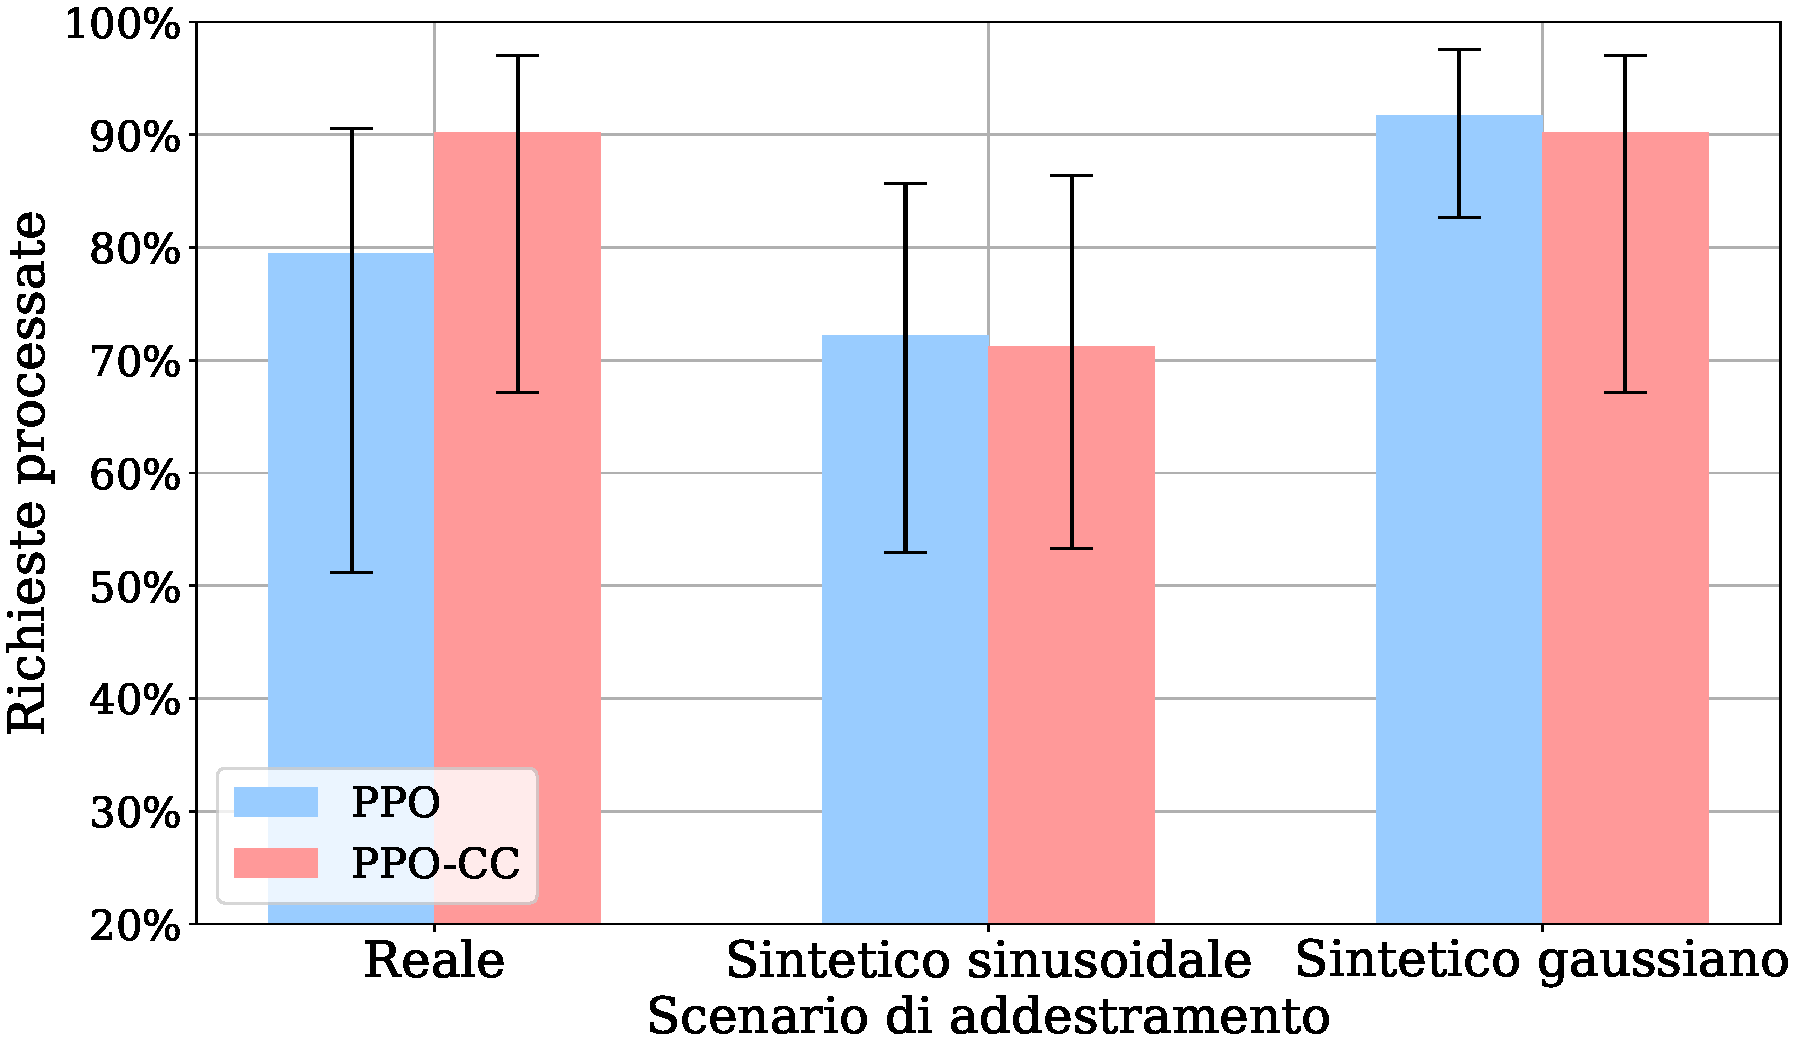
\includegraphics[width=\textwidth]{assets/5/results/eval_ASYM_summary_processed_requests.pdf}
    %         Ambiente ``ASYM''
    %     \end{column}
    %     \begin{column}{.35\textwidth}
    %         \centering
    %         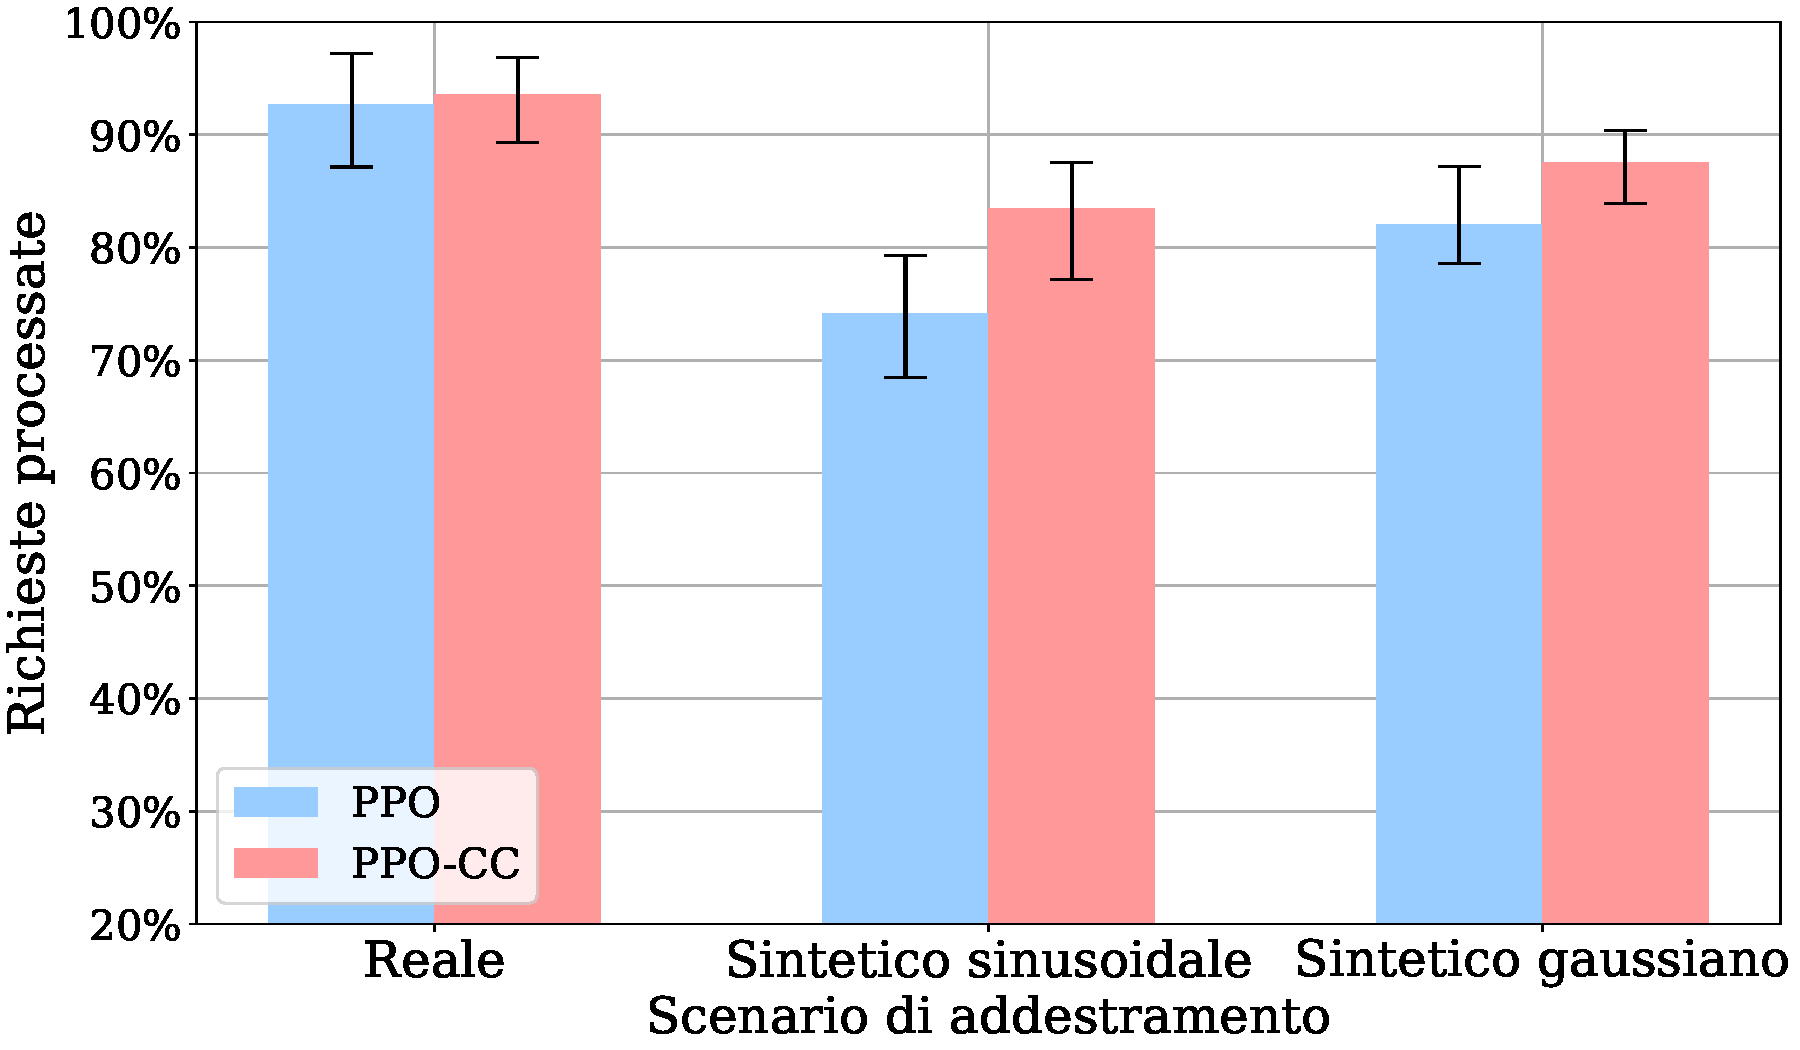
\includegraphics[width=\textwidth]{assets/5/results/eval_SYM_summary_processed_requests.pdf}
    %         Ambiente ``SYM''
    %     \end{column}
    % \end{columns}
    \begin{columns}
        \begin{column}{.5\textwidth}           
            \centering
            \small Ambiente ``BASE''
            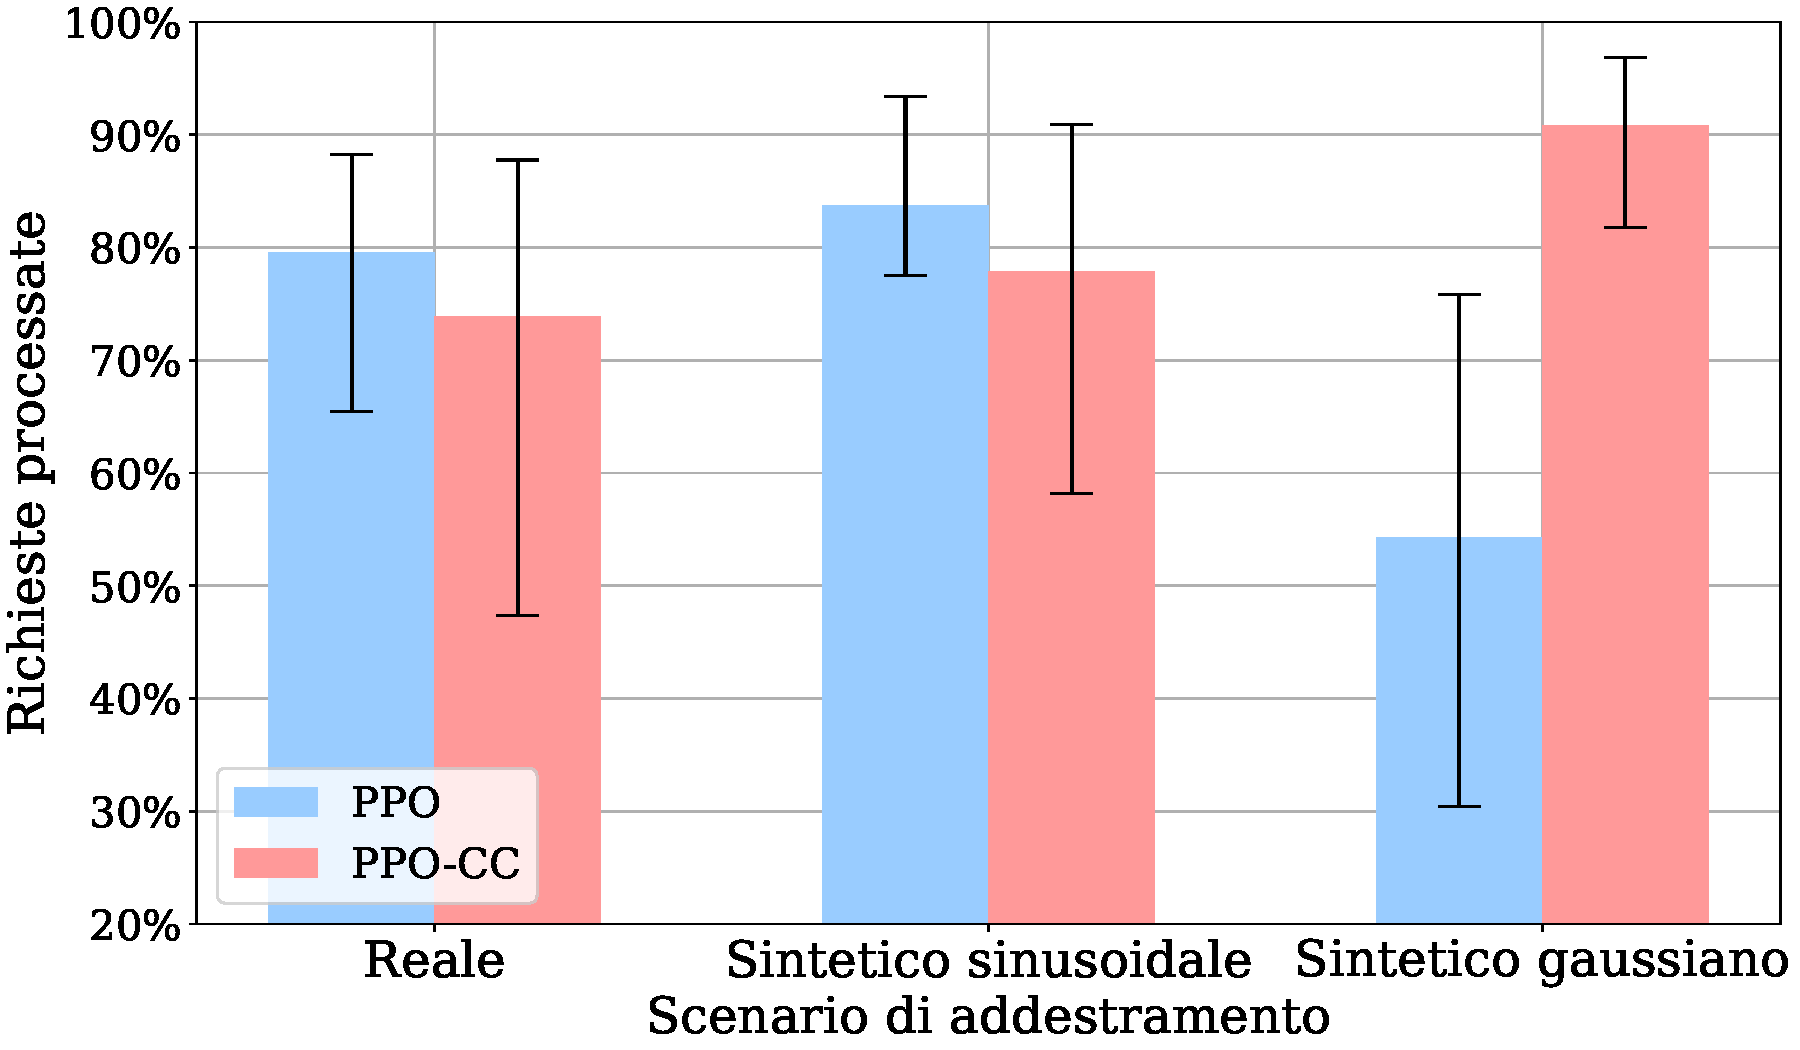
\includegraphics[width=6cm]{assets/5/results/eval_BASE_summary_processed_requests.pdf}
        \end{column}
    \end{columns}

    \vspace{.3cm}

    \begin{columns}
        \begin{column}{.5\textwidth}
            \centering
            \small Ambiente ``ASYM''
            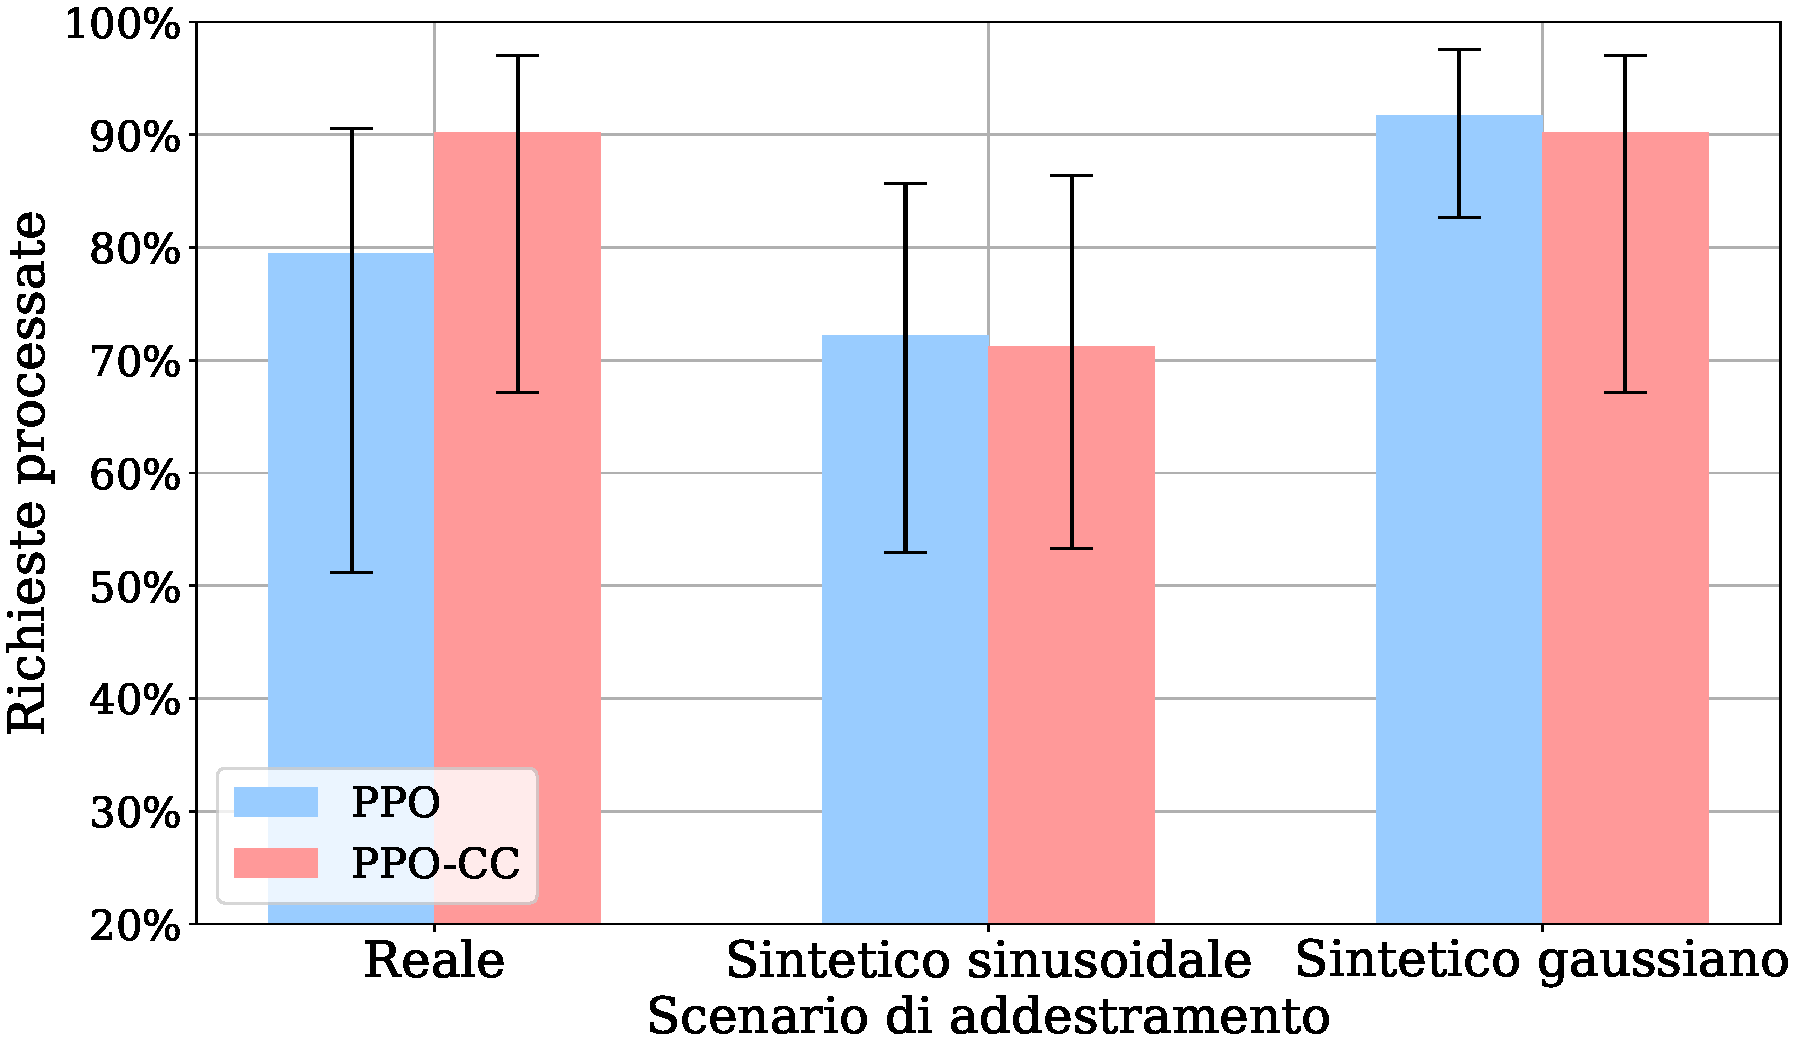
\includegraphics[width=6cm]{assets/5/results/eval_ASYM_summary_processed_requests.pdf}
        \end{column}
        \begin{column}{.5\textwidth}
            \centering
            \small Ambiente ``SYM''
            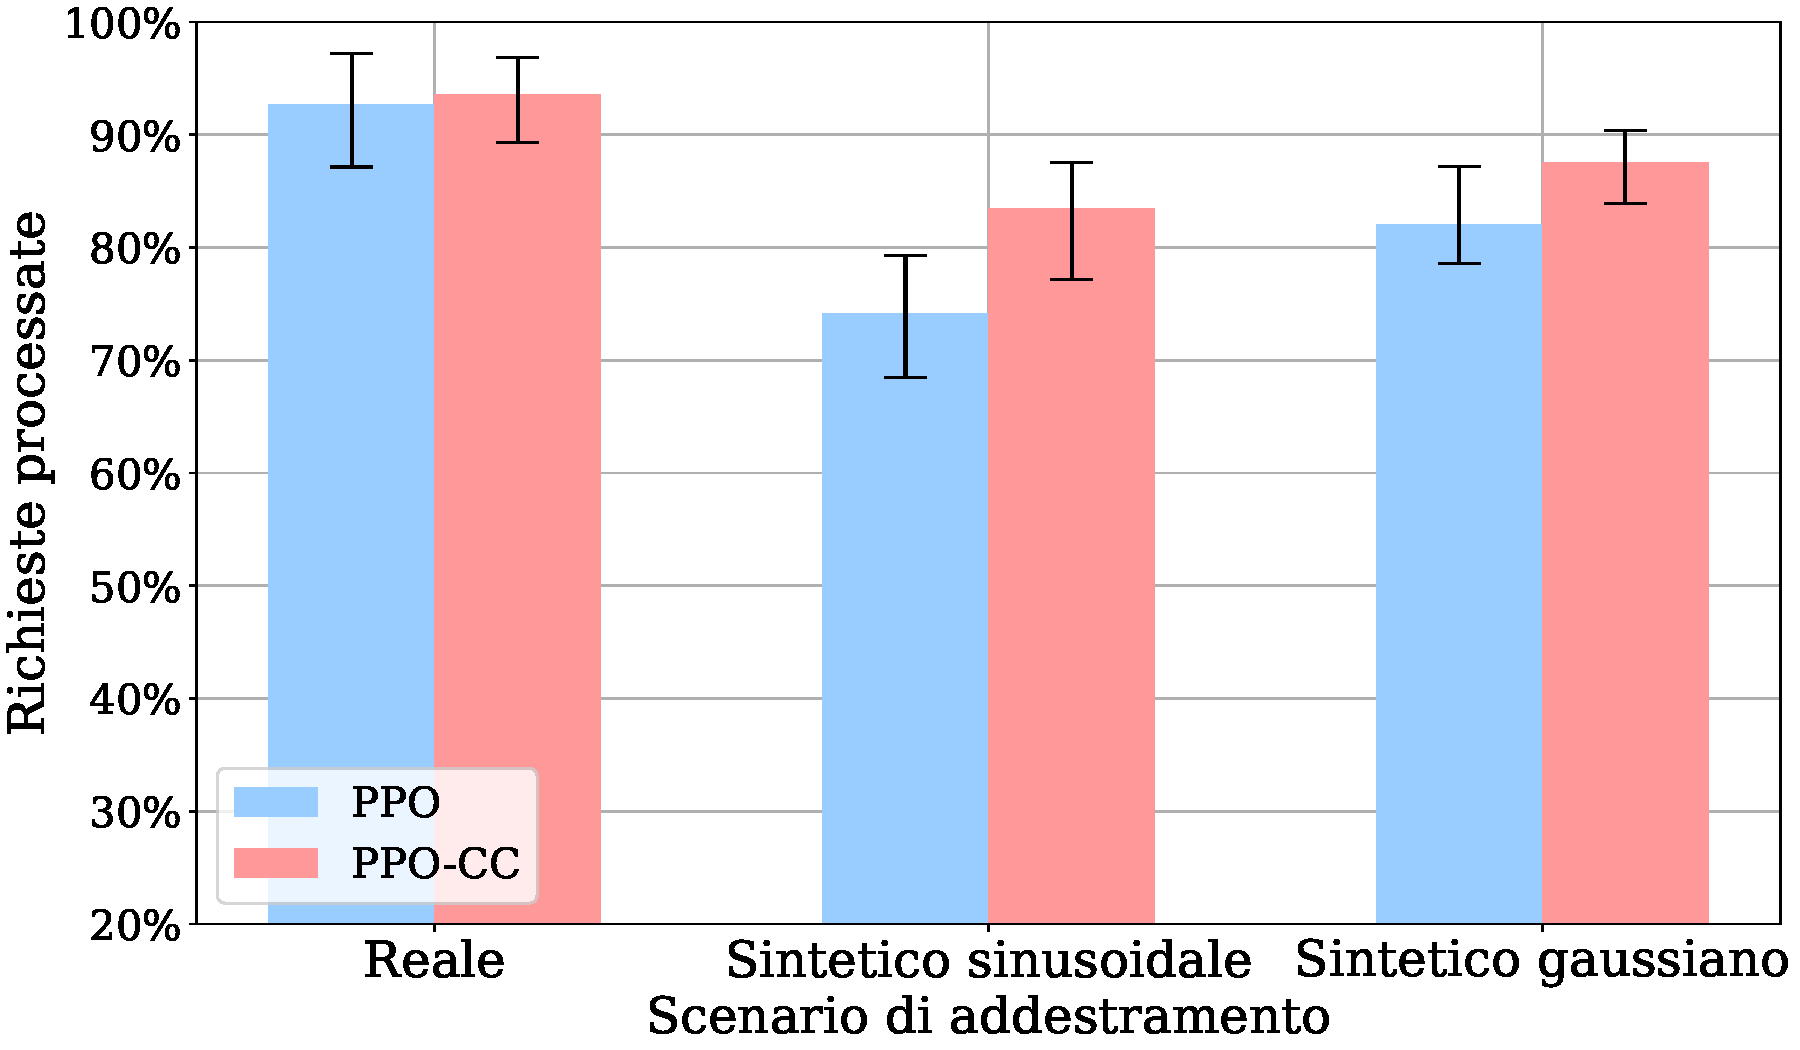
\includegraphics[width=6cm]{assets/5/results/eval_SYM_summary_processed_requests.pdf}
        \end{column}
    \end{columns}
\end{frame}

\begin{frame}{Richieste processate SYM su scenario reale}
    \centering
    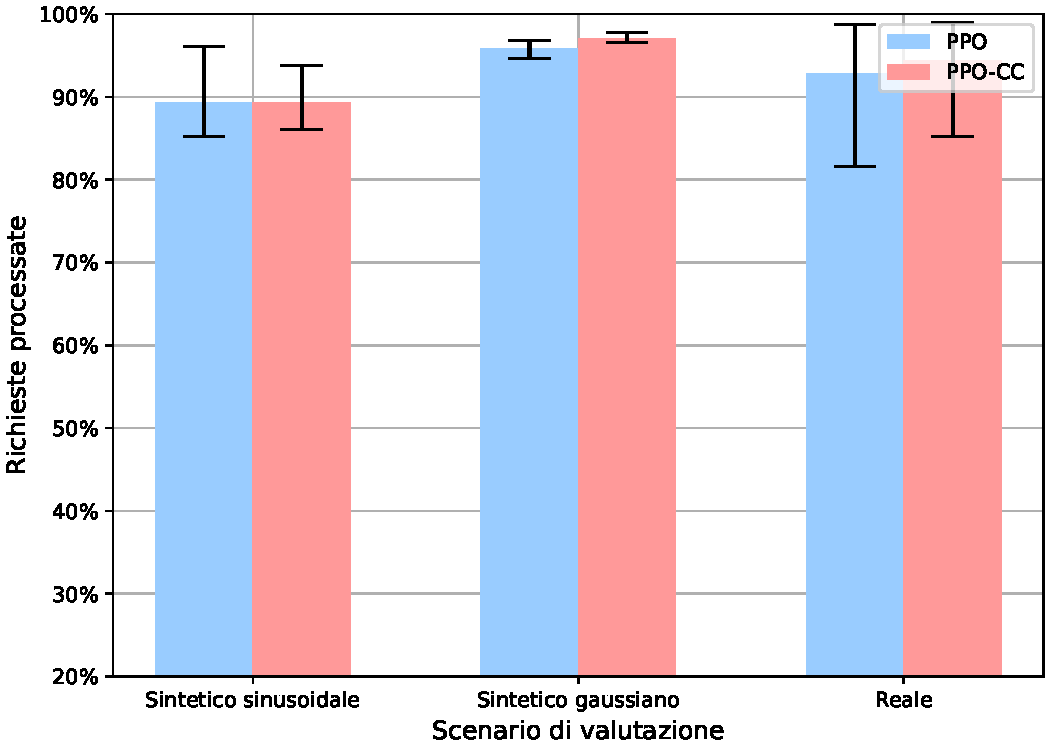
\includegraphics[width=.8\textwidth]{assets/5/results/eval_SYM_train_real_processed_requests.pdf}
\end{frame}

\section{Conclusioni}
    
\begin{frame}{Conclusioni}
    \begin{itemize}
        \item L'approccio MARL può affrontare il problema di distribuzione del carico in ingresso in ambienti edge-FaaS.
        \begin{description}
            \item[$\rightarrow$] L'inoltro migliora la gestione complessiva
            \item[$\rightarrow$] Condividere la rete Critic aiuta gli agenti a scegliere azioni migliori
        \end{description}

        \medskip

        \item Sviluppi futuri:
        \begin{itemize}
            \item Modellazione di un ambiente più simile a DFaaS reale
            \item Incentivare la cooperazione tra agenti
            \item Tuning iperparametri per PPO
            \item Uso di reti neurali con memoria (RNN)
        \end{itemize}
    \end{itemize}
\end{frame}

% Braces are necessary to keep background color only for this frame.
{
    \setbeamercolor{background canvas}{bg=unimib-discoGreen}
    \usebeamerfont{title}

    \begin{frame}[plain]
        % The two vfills are needed because the default alignment does not correctly vertical align the title.
        \vfill
        \centering
        \color{white} \huge Grazie per l'attenzione!
        \vfill
    \end{frame}
}

\appendix
\section{Appendici}

\begin{frame}{Ricompensa media totale}
    % \begin{columns}
    %     \begin{column}{.35\textwidth}
    %         \centering
    %         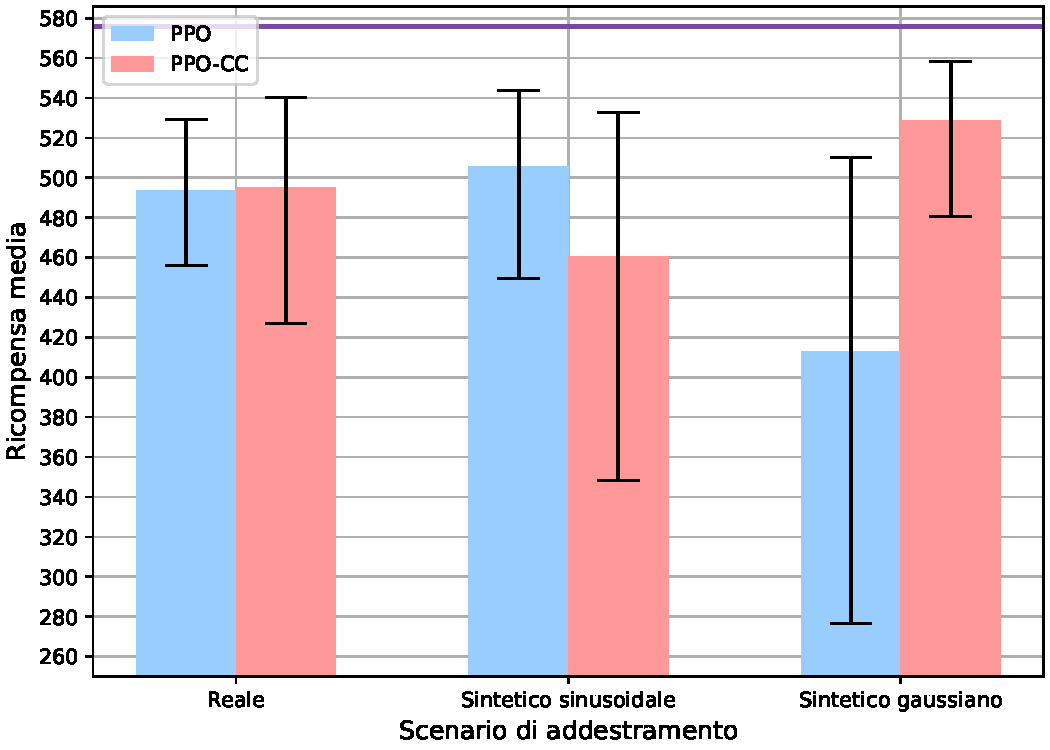
\includegraphics[width=\textwidth]{assets/5/results/eval_BASE_summary_reward.pdf}
    %         Ambiente ``BASE''
    %     \end{column}
    %     \begin{column}{.35\textwidth}
    %         \centering
    %         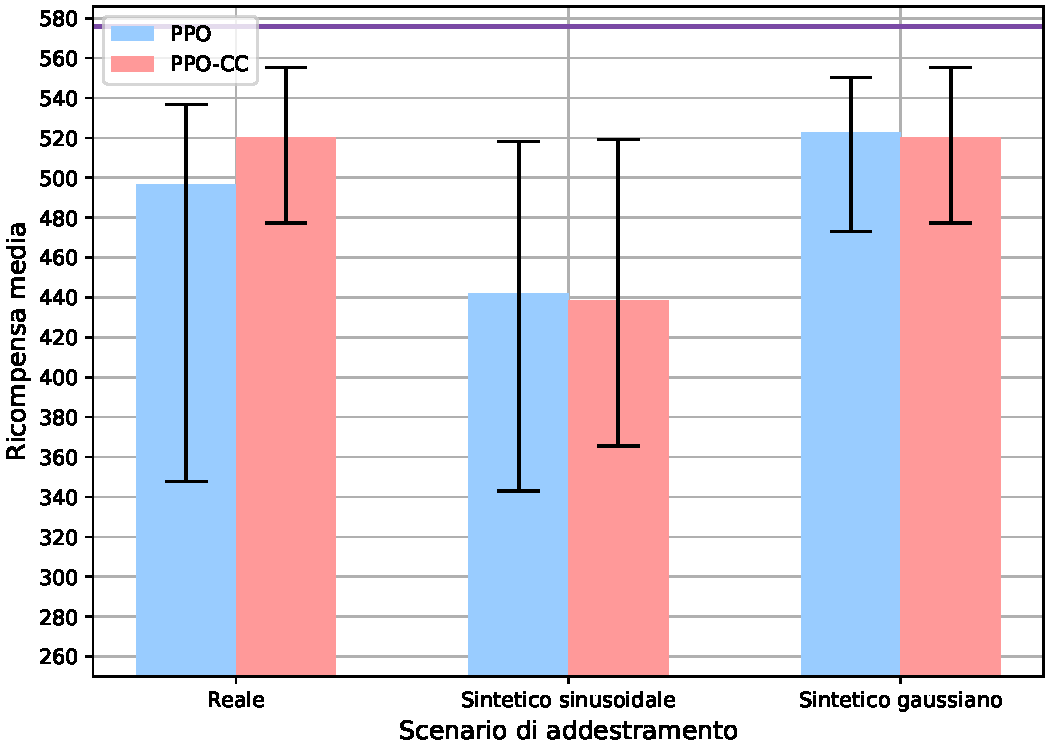
\includegraphics[width=\textwidth]{assets/5/results/eval_ASYM_summary_reward.pdf}
    %         Ambiente ``ASYM''
    %     \end{column}
    %     \begin{column}{.35\textwidth}
    %         \centering
    %         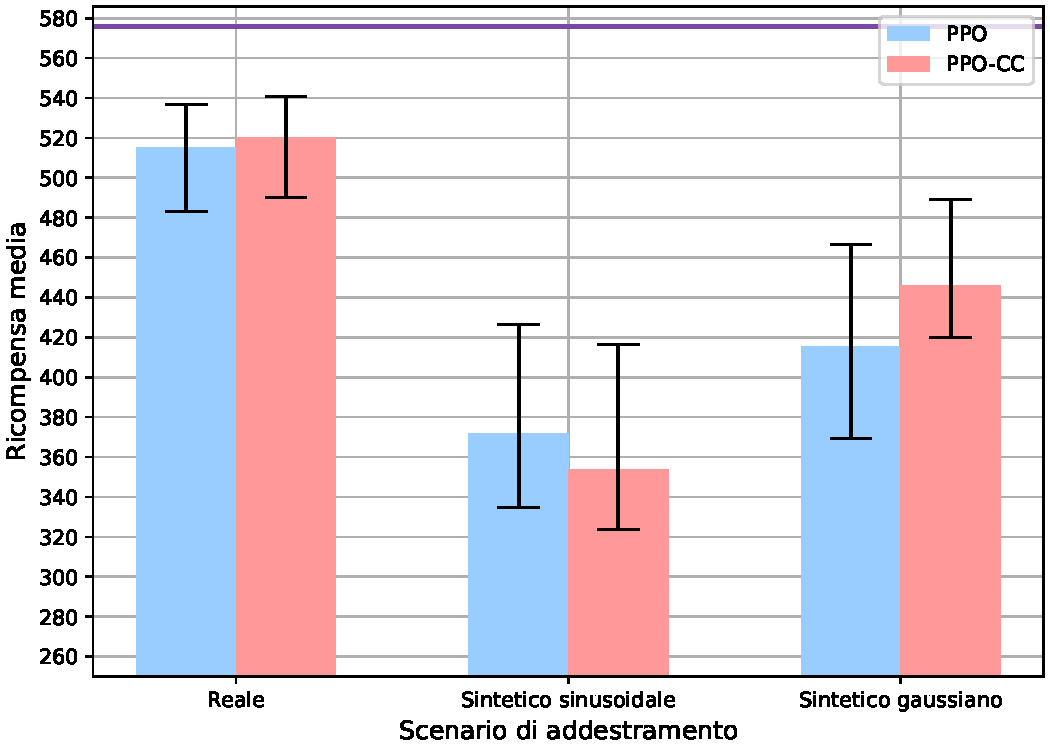
\includegraphics[width=\textwidth]{assets/5/results/eval_SYM_summary_reward.pdf}
    %         Ambiente ``SYM''
    %     \end{column}
    % \end{columns}
    \begin{columns}
        \begin{column}{.5\textwidth}           
            \centering
            \small Ambiente ``BASE''
            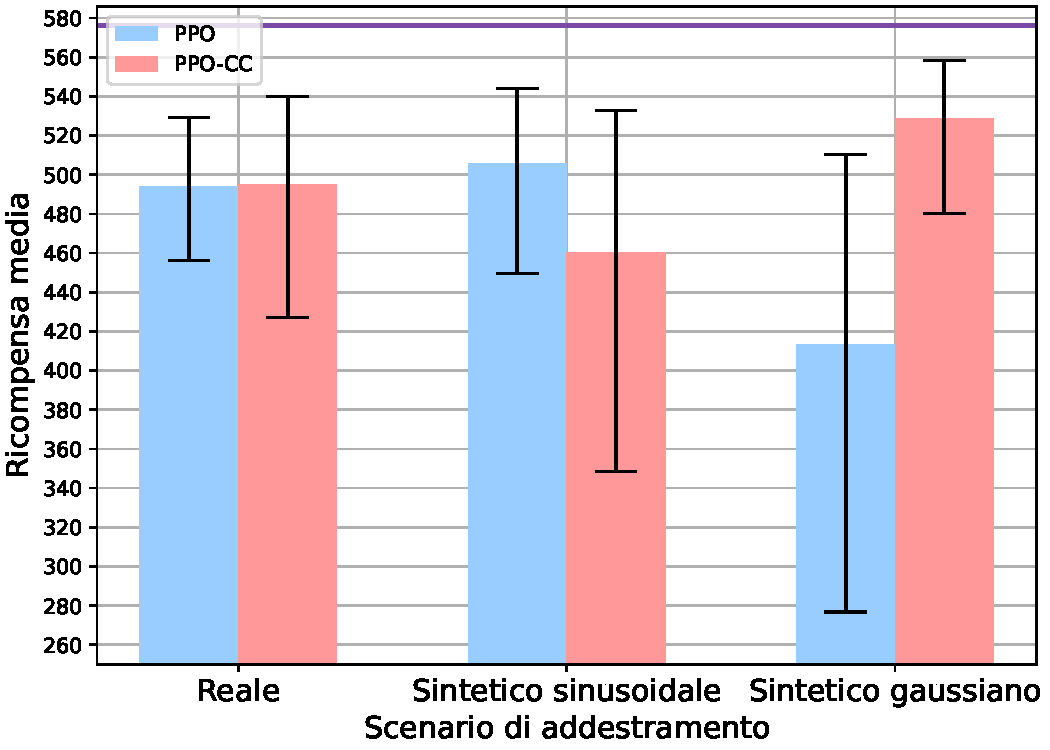
\includegraphics[width=5cm]{assets/slides/eval_BASE_summary_reward.pdf}
        \end{column}
    \end{columns}

    %\vspace{.3cm}

    \begin{columns}
        \begin{column}{.5\textwidth}
            \centering
            \small Ambiente ``SYM''
            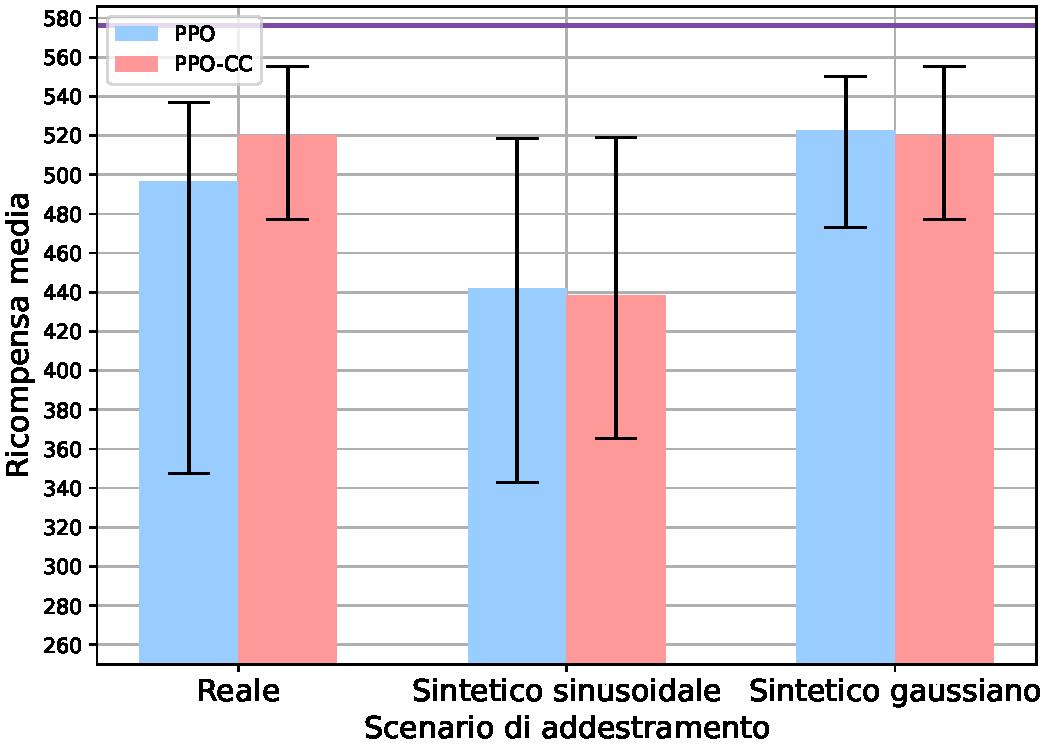
\includegraphics[width=5cm]{assets/slides/eval_ASYM_summary_reward.pdf}
        \end{column}
        \begin{column}{.5\textwidth}
            \centering
            \small Ambiente ``ASYM''
            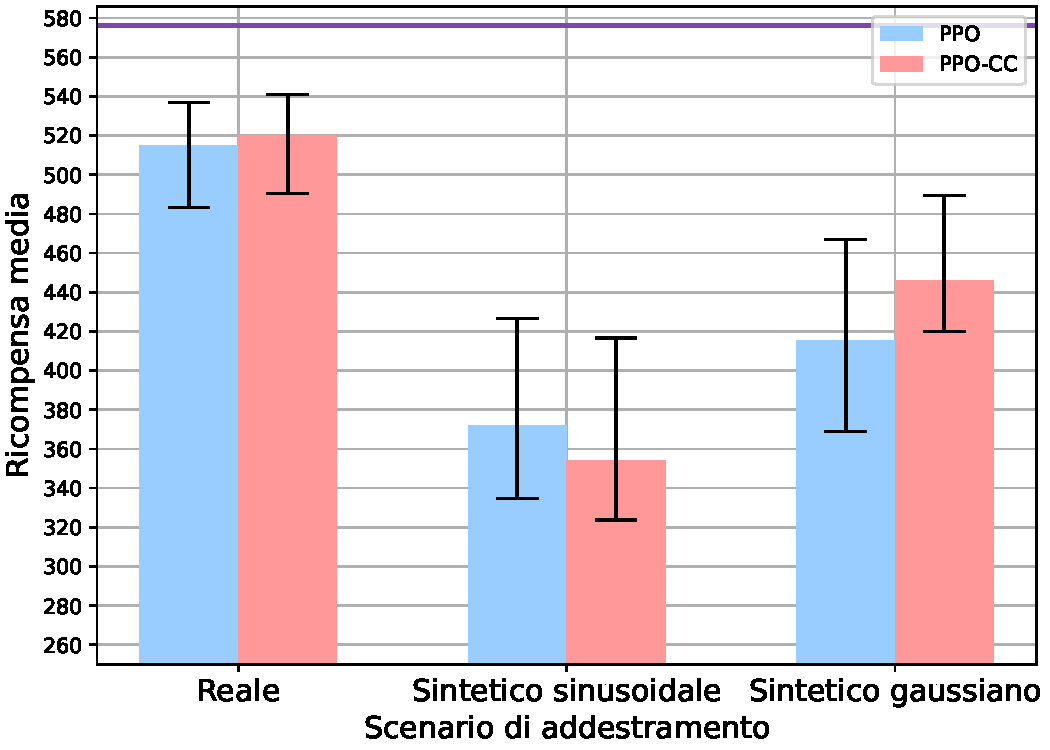
\includegraphics[width=5cm]{assets/slides/eval_SYM_summary_reward.pdf}
        \end{column}
    \end{columns}
\end{frame}

\begin{frame}{Richieste distribuite in ambiente SYM reale/reale PPO}
    \centering
    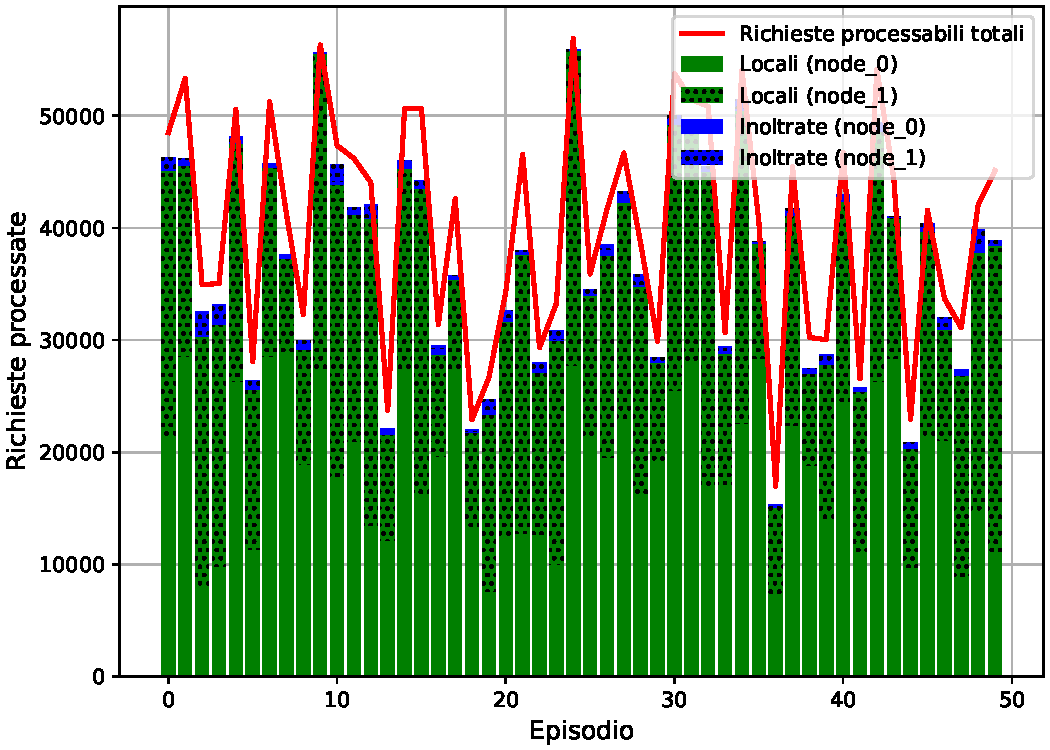
\includegraphics[width=.95\linewidth]{assets/5/results/real_real_ppo_proc_reqs_abs.pdf}
\end{frame}

\begin{frame}{Richieste distribuite in ambiente SYM reale/reale PPO-CC}
    \centering
    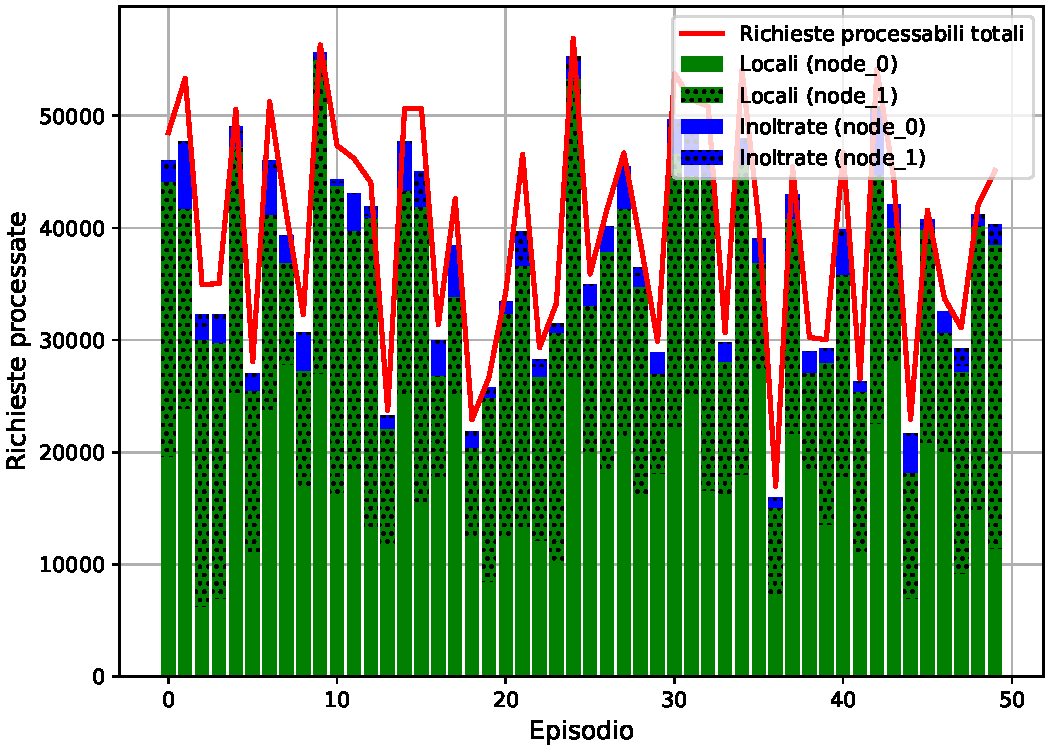
\includegraphics[width=.95\linewidth]{assets/5/results/real_real_ppo_cc_proc_reqs_abs.pdf}
\end{frame}

\end{document}